% Activate the following line by filling in the right side. If for example the name of the root file is Main.tex, write
% "...root = Main.tex" if the chapter file is in the same directory, and "...root = ../Main.tex" if the chapter is in a subdirectory.
 
% !TEX root = ../thesis.tex 

\chapter{Combined surface and volumetric Bayesian inference}
\label{svb_chapter}

\section{Introduction}

There are two dominant strategies for analysing volumetric data in a surface-based manner. One strategy is to process the data in volume space to obtain parameters of interest and then project these onto the cortical surface, whereas the other is to project the data itself onto the surface and then obtain the parameters of interest in that space. The appropriateness of each strategy is in part determined by the nature of the data in question. If the subcortex is assumed to contribute only noise signal, then projection onto the surface followed by noise reduction to remove said contribution is logical. This is the strategy adopted by the HCP for BOLD data in the \textit{fMRISurface} pipeline \cite{Glasser2013}. Conversely, if the subcortex does contribute a signal of interest in its own right, then it is more appropriate to attempt to separate out the different contributions in volume space before projecting only the cortical component onto the surface. For ASL data, this implies volumetric PVEc followed by surface projection, a strategy demonstrated by \cite{Verclytte2015}. Nevertheless, as was established in chapters \ref{lit_review_chapter} and \ref{pvec_chapter}, the drawback of this route is that volumetric processing may be fundamentally ill-suited to the anatomy of the cortex. 

The subject of this chapter is the development of a new approach that enables simultaneous surface and volumetric inference on data that contains both cortical and subcortical components. The motivation of this approach, named \textit{hybrid inference}, is to overcome the inherent limitations of volumetric approaches by estimating parameters of interest in the space to which they are most suited: cortical parameters are estimated in a surface-based manner and subcortical parameters in a volumetric manner. The result of this is a set of parameter maps in their respective spaces; unlike the volumetric approach, no further processing is required to project the results onto the surface. This approach has been implemented using an alternative formulation of variational Bayes to that embodied by FSL FABBER. 

\section{Stochastic variational Bayesian inference}

\subsection{Mathematical formulation}

As was previously set out in section \ref{lit_vb}, the objective of VB inference is to derive an optimal approximation to a posterior\footnote{The formulation of stochastic variational Bayesian inference presented in this section was originally published as M. Chappell, M. Craig and M. Woolrich, ``Stochastic Variational Bayesian Inference for a Nonlinear Forward Model", arXiv e-prints, 2020, doi: arXiv:2007.01675. What follows in the remainder of this chapter are the modifications and extensions that were made to that work to enable surface and hybrid inference, all of which are original.}. FABBER's implementation of VB uses an analytic approach to perform optimisation. In particular, application of the calculus of variations to the objective function, given the parametric form of the likelihood and priors, yields a set of update equations that are iteratively applied until convergence is reached. This approach means that the update equations are specific to the parametric form of model and priors in question; if any of these are modified, then the updates must be re-derived from scratch. This property explains the importance of the conjugate-prior restriction, for example, which greatly simplifies the derivation of updates. 

VB need not be tied to this specific optimisation method and could in fact be made to operate under any suitable framework. In turn, this would allow some of the restrictions that facilitate the calculus of variations to be relaxed; for example the linearisation of non-linear models or the requirement of conjugate-prior distributions \cite{Chappell2009}. The implementation presented in this chapter starts by considering the expression for free energy, which is the objective measure of approximation quality that is sought to be optimised. 

\begin{equation}
\label{free_energy}
F(\theta) = \int q(\theta) \log \left( p(y|\theta) \frac{p(\theta)}{q(\theta)} \right) d\theta
\end{equation}

In the above equation, $p(y|\theta)$ is the likelihood, a property of the generative model $g(\vec{\theta})$ that is being fit to the data, $p(\theta)$ is the prior, and $q(\theta)$ is the approximation to the true posterior. Conceptually, there are two separate contributions to the free energy. The first of these is a reconstruction loss, which describes how well the parameter estimates reconstruct the observed data; the second is a latent cost that describes how far the parameter estimates deviate from the prior. The VB strategy is to parameterise $q$ in terms of some hyper-parameters $\psi$, which leads to $q(\theta; \psi)$. Whereas analytic VB would at this point use the calculus of variations to derive a series of update equations on $\psi$ to perform the optimisation, the stochastic approach takes the more direct approach of gradient descent. To do so, the gradients with respect to the hyper-parameters are required: 

\begin{equation}
\nabla_{\psi} F(\theta) = \nabla_{\psi} \left[ \int q(\theta) \log \left( p(y|\theta) \frac{p(\theta)}{q(\theta)} \right) d\theta \right]
\end{equation}

Direct evaluation of the gradients is generally infeasible in practice, but a sampling approach may instead be used. For example, a Monte Carlo approximation for the free energy (equation \ref{free_energy}) yields: 

\begin{equation}
\label{free_energy_approx}
F \approx \frac{1}{L} \sum^{L}_{l} \left[ \log( p(y|\theta^{*l}) ) - \log \left( \frac{q(\theta^{*l})}{p(\theta^{*l})} \right) \right]
\end{equation}

In this approximation, the integral is constructed as the average across $L$ samples of $\theta$. Each sample $\theta^{*l}$ is drawn from the approximate posterior $q(\theta)$. The gradient can then be calculated on this approximation. 

\begin{equation}
\nabla_{\psi} F \approx \frac{1}{L} \sum^{L}_{l} \nabla_{\psi} \left[ \log( p(y|\theta^{*l}) ) - \log \left( \frac{q(\theta^{*l})}{p(\theta^{*l})} \right) \right]
\end{equation}

This equation represents the basis for performing VB via \textit{stochastic} gradient descent, an approach hereafter referred to as stochastic variational Bayes (SVB). Note that although the gradient is calculated on an \textit{approximation} of the free energy, the calculation of the gradient itself is performed analytically. This is made possible via automatic differentiation across a computational graph. 

The inherent risk of a sampling-based approach is that the gradient estimates may be noisy, which in turn could frustrate convergence of the optimisation. In some regards, this could be seen as advantageous as some level of stochasticity may help explore the parameter space and avoid local minima. However, it may also lead to poor convergence as the gradient estimates are highly variable, in particular due to the fact the samples themselves are a function of the \textit{current} value of $\psi$. If $\psi$ is far from optimality, then it is possible that the samples drawn from $q(\theta)$ will produce a poor approximation of the true gradient in $\psi$-space. 

Within the field of machine learning, this challenge has been addressed via the use the \textit{reparameterisation trick} \cite{Kingma2013}. In this formulation, $\theta$ is expressed as a function of a random variable $\epsilon$ with a distribution that does not depend on $\psi$. The motivation is to ensure the distribution of samples of $\theta$ can be decoupled from $\psi$; hence with a suitable choice of distribution, samples of $\theta$ are more likely to cover parameter space resulting in more accurate gradient estimates. 

A general means of implementing reparameterisation is to exploit the probability integral transform. Samples of a random variable from an arbitrary probability density function will be uniformly distributed when transformed by the cumulative density function (CDF). Thus, a sample of $\epsilon$ can be converted into a sample of $\theta$ via

\begin{equation} 
\theta^* = \mathrm{CDF}^{-1}_{\psi} \left( \Phi(\epsilon) \right)
\end{equation}

where $\Phi(\epsilon)$ is the CDF for the standard normal and $\mathrm{CDF}^{-1}_{\psi}$ is the inverse CDF for $\psi$. In this expression, the standard normal (zero mean and unit variance) has been chosen as the distribution for $\epsilon$ as it is convenient to sample. Similarly, if $q(\theta)$ is taken to be a multivariate normal (MVN) distribution, then the inverse CDF is readily obtained. 

The final two components that are required for SVB are expressions for the model likelihood $p(y|\theta)$ and prior $p(\theta)$. The former will be dealt with here, and the latter will be discussed separately in section \ref{svb_spatial_prior}. The inference problem for a nonlinear model $g$ can be written as 

\begin{equation}
\vec{y} = g(\vec{\theta}) + \vec{e} 
\end{equation}

where $\vec{y}$ is a vector of acquired data of length $N$, with $N$ the number of samples acquired, $g$ is a non-linear generative model with parameters $\theta$, and $\vec{e}$ is a vector of noise contributions of length $N$. Under the assumption of white Gaussian noise $\vec{e} 
\sim N(0, \rho)$, the log-likelihood across $N$ observations is 

\begin{equation}
\log p(\vec{y} | \Theta) = \frac{N}{2} \log \rho - \frac{\rho}{2} (\vec{y} - g(\theta))^T (\vec{y} - g(\theta))
\end{equation}

where $\Theta = \{ \theta, \rho \}$ is the set of all model and noise parameters. In this work, an MVN distribution over $\Theta$ is used to approximate the true posterior. Accordingly,  

\begin{equation}
q(\Theta) = q \left( \begin{bmatrix} \theta \\ -\log(\rho) \end{bmatrix} \right) = N(\Theta; \vec{m}, \mat{C})
\end{equation}

where the noise precision (inverse variance) is inferred on a log-scale to restrict it to positive values only. This formulation allows for covariance between model parameters, something which was not possible under the analytic formulation of VB. The use of an MVN also lends itself readily to the incorporation of reparameterisation gradients, namely via

\begin{equation}
\Theta^* = \vec{m} + \mat{S}\epsilon^* 
\end{equation}

where $\epsilon \sim N(0,\mat{I})$ and S is the Cholesky decomposition of $\mat{C} = \mat{SS^T}$. For the work presented here relating to inference on ASL data, independence of the kinetic model parameters $\theta$ has been assumed. This means the covariance matrix $\mat{C}$ contains only diagonal entries. 

\subsection{Implementation}

SVB has been implemented using TensorFlow, a machine learning and optimisation library that uses a computational graph model \cite{abadi2016}. The expression for free energy is constructed as a network of discrete mathematical operations and edges that represent the flow of data between them. Efficient calculation of gradients across the network is made possible due to the use of automatic differentiation (also referred to as back-propagation in the machine learning literature). Within TensorFlow, the optimisation itself is performed using the Adam algorithm, a variant of stochastic gradient descent that is suited to high dimensional data and that incorporates a number of features that improve robustness to local minima \cite{Bottou2010, adam_optimisation}. 

Prior to this work, SVB had been developed and published for volumetric inference only \cite{chappellSVB, chappell2020fmrib}; broadly speaking, this may be regarded as equivalent to FABBER except in the means by which optimisation is performed. What follows in the remainder of this chapter are the set of modifications that were made to volumetric SVB in order to enable hybrid inference. 

\section{Spaces of inference}

SVB has been extended to perform inference in a number of different spaces. The term \textit{nodes} is used to refer to the spatial locations within each space at which parameter estimation is performed. A space of inference is defined by the following characteristics: a set of nodes at which inference is to be performed, a projection from nodes to voxels that allows volumetric data to be reconstructed from node values, and an implementation of the spatial prior within node space. The form of the spatial prior within each space will be discussed separately in the following section. 

\subsubsection{Volume}

This space provides conventional voxel-wise inference in a manner equivalent to FABBER. The set of nodes is simply the set of all voxels and the projection to volume space is the identity transform.  

\subsubsection{Surface}

This space provides inference for the cortex in a manner that does not acknowledge the potential existence of subcortical contributions within the data. This would be appropriate for a modality for which the subcortex does not contribute substantial signal (notably, BOLD). In this case, the set of nodes contains the vertices of each cortical hemisphere and the projection to volume space is made using Toblerone's framework. 

\subsubsection{Region of interest}

This space provides inference for regions of interest (ROI) that are known to cover multiple contiguous voxels. The specific use case in mind are the subcortical structures identified by FSL FIRST (\textit{e.g.}, putamen, caudate and thalamus) though in principle any arbitrary ROI could be used. Regions of interest are defined by a volumetric PV estimate mask, which may optionally be generated directly using the method presented in chapter \ref{tob_pv_chapter} if suitable surface segmentations are available (for example, from FIRST). ROIs are treated in an averaging manner: all voxels within the ROI map onto a \textit{single} node representing the entire region, in proportion to their respective PVs. Projection to and from this space is achieved within the Toblerone framework by concatenating a row or column to the appropriate surface or hybrid projection matrix. 

\subsubsection{Hybrid}

This space represents the union of the volumetric, ROI and surface spaces, resulting in \textit{simultaneous} inference for all of them. In keeping with the convention adopted by the HCP within the CIFTI file format \cite{Glasser2013}, the set of all nodes is defined (in order) as left hemisphere vertices, right hemisphere vertices, subcortical voxel centres, and ROIs sorted in alphabetical name order. The projection to volume space is made using Toblerone's framework. 

The defining characteristic of hybrid space is that each node represents only a single tissue (\textit{i.e.}, a region of cortex, a subcortical ROI, or subcortical WM). This is different to volume space in which a single node (corresponding to a single voxel) may contain and therefore represent multiple tissues. In hybrid space, a voxel that contains multiple tissues will by definition map onto multiple nodes (vertices for the cortex, voxel centres for the subcortex) that represent exactly one tissue class each. The overall schematic for the optimisation performed by SVB in hybrid space is shown in figure \ref{svb_schematic}.

\begin{figure}
\centering
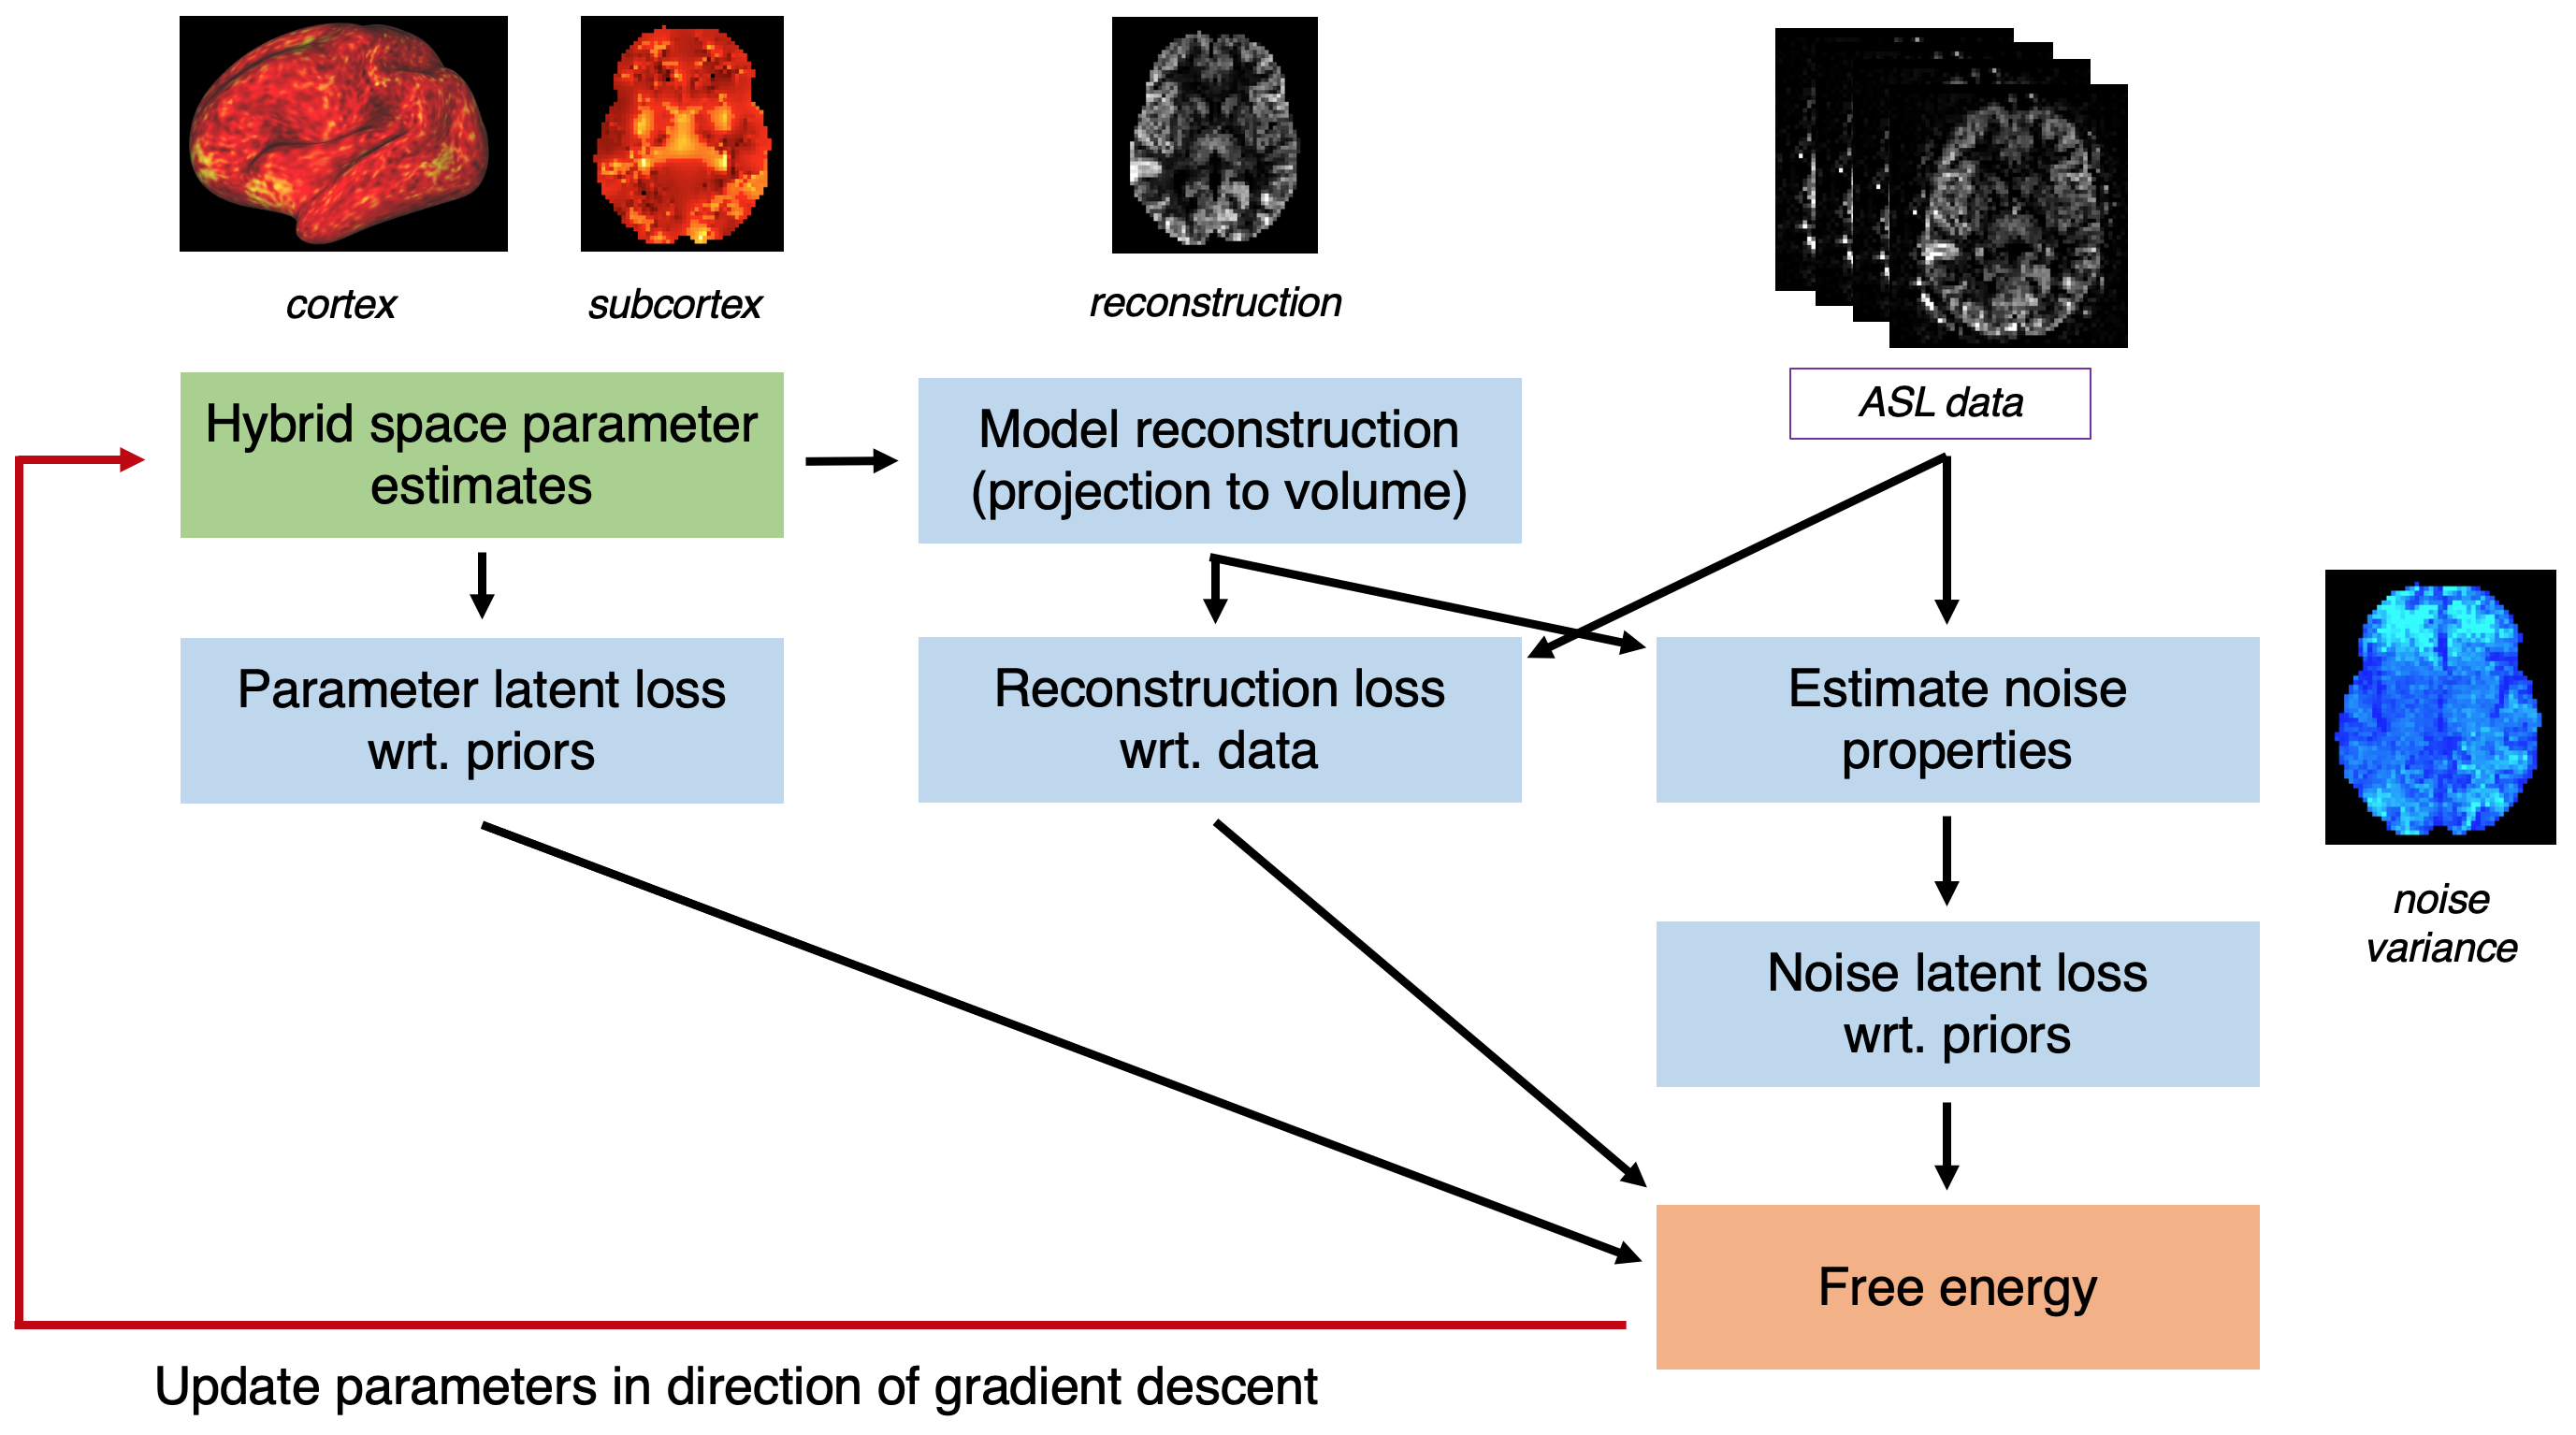
\includegraphics[width=\textwidth]{svb_schematic.png}
\caption{The optimisation loop that is the heart of SVB hybrid inference. Each iteration starts at the box shaded in green and terminates at the box shaded orange; the gradient in cost is then calculated and the parameter estimates updated in light of this for the next iteration. The ASL data is constant and external to the loop. For hybrid inference, the two key stages are i) model reconstruction, which involves a projection from nodes to volume space, and ii) noise estimation in the \textit{volume} space only.}
\label{svb_schematic} 
\end{figure}

Volumetric PVEc under BASIL is performed as an optional post-processing step that attempts to fit a kinetic model with GM and WM components in every voxel, regardless of whether a voxel actually contains the tissue in question. This leads to the slightly paradoxical outcome of estimating GM CBF deep in the subcortex, for example, even though GM may not locally be present (the paradox is resolved by assigning the GM estimate zero weight in the reconstruction step). By contrast, such redundancy does not arise within hybrid space because it is known ahead of time that each node represents a single tissue, and combined with Toblerone's PV-aware projection framework, this means PVEc is intrinsic to the inference process. In fact, it would be impossible to perform inference in hybrid space via the Toblerone projection framework \textit{without} also performing PVEc.

\subsubsection{The Toblerone projector}
\label{tob_projector_paragraph}

The surface, ROI and hybrid spaces use Toblerone's projection framework in order to reconstruct volumetric data from their respective node-wise parameter estimates. From an implementation point of view, this is embodied in the concept of a \textit{projector}, a software object that encapsulates all of the matrices and PV estimates required to project from the space of inference back into an arbitrary voxel grid. \textit{Initialising a projector} is done using a set of cortical and subcortical surfaces, ROI definitions, a registration that maps these into alignment with the data at hand, and the voxel grid of the data itself. This operation may be regarded as roughly equivalent to a PV estimation step within a conventional volumetric analysis pipeline. For the remainder of this chapter, any reference to performing SVB inference in the surface or hybrid space also implies the use of a Toblerone projector. 


\section{Incorporation of the spatial prior}
\label{svb_spatial_prior}

The role of the spatial prior within VB is to enforce similarity of parameter estimates between spatially proximate nodes\footnote{This is separate and distinct to a distributional prior that considers individual parameter values in isolation (for example, with respect to a normal distribution of known mean and standard deviation). At the time of writing, this means that one must choose between a spatial or distributional prior within the VB framework, and though attempts have been made to unify the two types together, implementation of such a combined spatial and distributional prior remains challenging \cite{Groves2009a}.}. This serves two related but distinct purposes: noise rejection and conditioning for PVEc. The first is desirable due to the intrinsically low SNR of ASL data. The second is obligatory to enable PVEc: as estimation of kinetic curves for both GM and WM using a single voxel timeseries of data is inherently under-determined, the spatial prior allows for the incorporation of neighbourhood data to better condition the problem. Within the VB framework, the prior is expressed as a latent cost that measures the degree of dissimilarity between neighbouring nodes. The logarithm of latent cost associated with the application of the spatial prior over a \textit{single} model parameter $\theta_i$ may be expressed as follows.  

\begin{equation}
\log{P} = \frac{1}{2}\log{\phi} - \frac{\phi}{2}\theta_i^T\mat{D}\theta_i + \log{Ga(\phi)}
\end{equation}

\begin{equation}
\log{Ga(\phi)} = (q_1 - 1) \log{\phi} - \frac{\phi}{q_2} 
\end{equation}

In the above expressions, $\theta_i$ is a vector of node-wise parameter estimates, $\mat{D}$ is a matrix operator that encodes neighbourhood information, and $\phi$ is the spatial precision, the weight that is given to the spatial prior. The spatial precision $\phi$ is a target of the optimisation itself (sitting one level above the physiological parameters in the Bayesian hierarchy); larger values represent increased levels of smoothing. Both FABBER and SVB use the Laplacian matrix for $\mat{D}$. The two key quantities of interest in these expressions are $\frac{\phi}{2}\theta_i^T\mat{D}\theta_i$, which evaluates the sum of squared differences (SSD) across each neighbourhood of nodes, and $\log{Ga(\phi)}$, which represents a prior on the value of $\phi$ itself. The SSD term measures the extent of dissimilarity in $\theta_i$: any vector that does not contain perfectly homogenous values will produce a strictly positive SSD if $\mat{D}$ is positive semi-definite. The contribution of this to the overall latent cost scales linearly with $\phi$. The prior on $\phi$ itself, represented by a Gamma distribution $Ga(\phi)$, leads the optimisation to prefer minimal levels of smoothing. Without this prior, it is possible to set up a positive feedback loop whereby the optimal response to a large $\phi$ value is to reduce variance in the parameter estimates, which in turn supports further increases in $\phi$, et cetera. 

The Gamma distribution on $\phi$ is parameterised by location $q_1$ and scale $q_2$ constants. With $q_1$ = 1, the distribution has a peak at $\phi$ = 0 and exhibits monotonic exponential decay; it is this property that causes the optimisation to prefer small values of $\phi$. Varying $q_2$ can be used to increase the width of the distribution (illustrated in figure \ref{gamma_q2_plot}), tolerating increased levels of smoothing without introducing bias. 

\begin{figure}
\centering
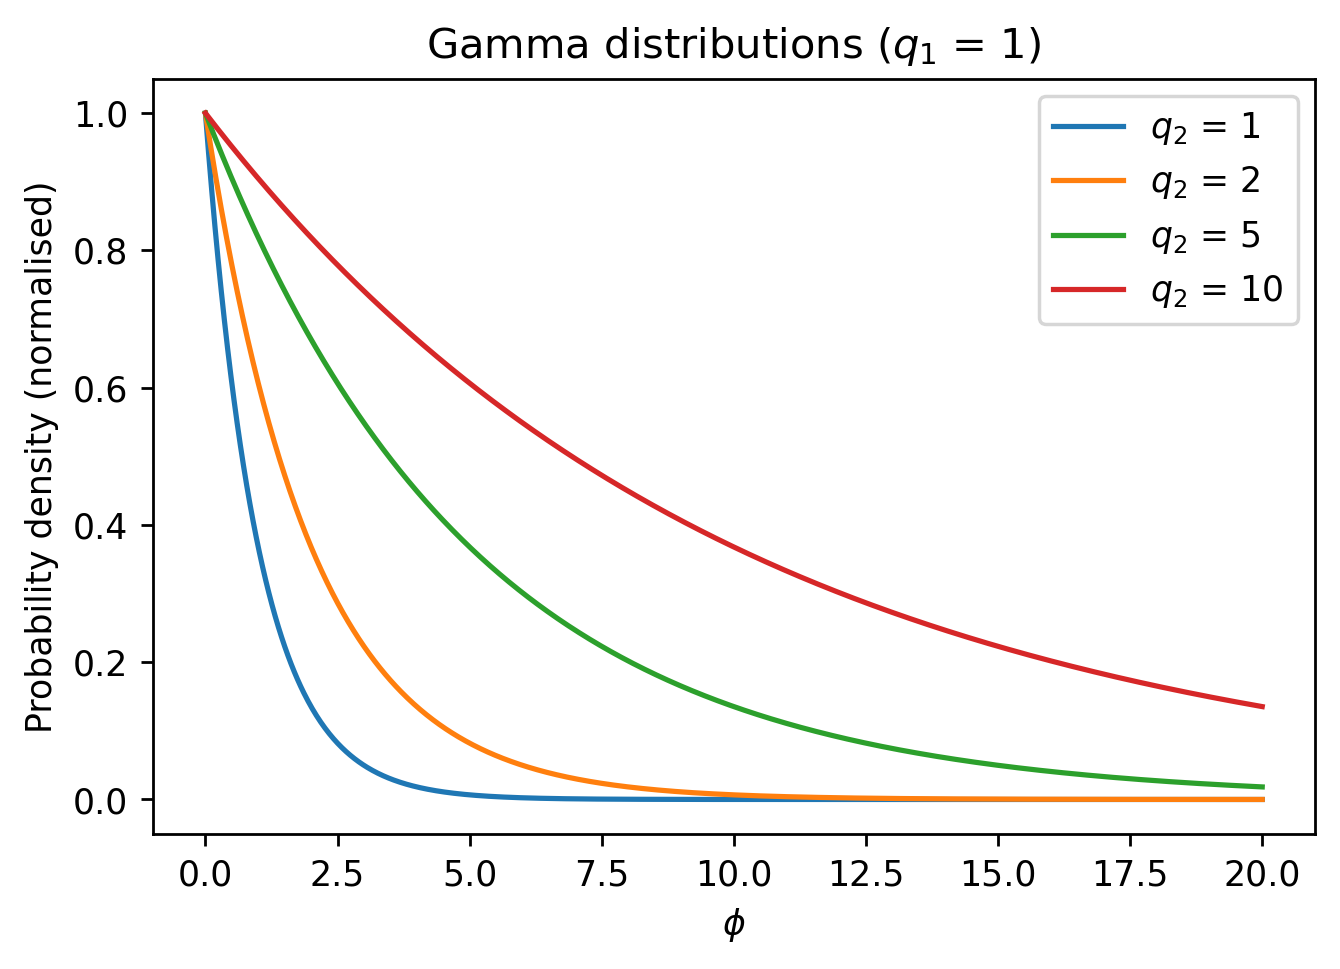
\includegraphics[width=0.6\textwidth]{gamma_q2_plot.png}
\caption{Probability density functions (normalised) for the Gamma distribution with $q_1$ = 1 and varying $q_2$. As $q_2$ increases, the width of the distribution increases, meaning higher values are relatively more probable.}
\label{gamma_q2_plot} 
\end{figure}

Within FABBER, the parameters of the Gamma distribution on $\phi$ are set at $q_1$ = 1 and $q_2$ = 10. These values were originally proposed by Penny \textit{et al.} when introducing the spatial prior to the VB framework, and were chosen to be relatively uninformative due to a lack of knowledge about what values $\phi$ might take. In fact, the authors stated that ``as we gather more experience applying such priors to fMRI data, we envisage, in the future, choosing $q_1$ and $q_2$ to reflect this knowledge" \cite{Penny2005}. During the development of hybrid SVB, it was found that using the same combination of Laplacian matrix and Gamma distribution as FABBER did not give good performance, so the modifications detailed in the following paragraphs were duly made. Note that in the case of subcortical ROIs, the spatial prior is not applied: as each ROI contains multiple voxels that are aggregated to yield a single parameter estimate, in effect a strong prior is already imposed in the inference process within said region.  

\subsection{Volume space}

In keeping with FABBER, the spatial prior in the volumetric space is encoded using a discrete Laplacian matrix. Whereas FABBER uses unity edge weights regardless of the true distances between voxels, inverse distance weighting was used for SVB to better handle the anisotropic voxel grids commonly found in ASL imaging. The matrix $\mat{D}$ was therefore defined as follows: 

\begin{equation}
  D_{i,j} =
  \begin{cases}
    0 & \text{for } j \notin N(i) \\
    d^{-n} & \text{for } j \in N(i) \\
    -\sum\limits_{k \in N(i)} D_{i,k} & \text{for } j = i 
  \end{cases}
\end{equation}

where $N(i)$ is the neighbourhood function for voxel $i$ that includes the six cardinal neighbours ($\pm$1 along each axis), and $d^{-n}$ is the geometric distance between voxels $i$ and $j$ weighted to the power $n =$ 1. Finally, the weight of a voxel to itself ($D_{i,i}$) is simply the negative sum of its weights to all other voxels, which ensures that the sum of weights for any voxel is zero. If extremely high noise rejection were required, it would be possible to extend the neighbourhood function to include other neighbours (diagonals, second-neighbours \textit{etc}); the six immediate neighbours along each axis have been found to give good performance for typical ASL data. 

\subsection{Surface and hybrid space}

Multiple variants of the Laplacian operator for surface meshes (summarised in table \ref{laplacian_table}) were investigated during development. The simplest of these, the mesh Laplacian, assigns unity weight to vertices directly connected by an edge, and assigns the weight of a vertex to itself as the negative sum of all other weights. This formulation can be extended to include inverse distance weighting in the same manner as for the volumetric case, which again will better account for the non-constant edge lengths found on cortical surface reconstructions. The matrix is constructed as for the volumetric case, except that the neighbourhood function instead records the existence of edges between vertices. If increased noise rejection were required, it would be possible to include second neighbours in the matrix, though care would need to be taken to ensure the distance weighting was performed using geodesic (along the surface) rather than geometric (straight-line) distance. To do otherwise would negate one of the key assumptions underpinning surface-based analysis, namely that areas of cortex will correlate better with geodesic distance than geometric. 

The Laplace-Beltrami operator (LBO) is a more sophisticated formulation that attempts to account for the area around each vertex that `belongs' to the respective edges \cite{Meyer2003}. As is the case with edge lengths, the angle around any vertex cannot be assumed to split equally amongst the triangles that contain that vertex; the LBO will assign a greater weight to those that account for a greater angle. Though the LBO is in common use within the field of computational geometry, it was deemed unsuitable for use in this application as it is not guaranteed to produce a semi-definite matrix. This means that the quantity $\theta_i^T \mat{D} \theta_i$ may not be of fixed sign for all $\theta_i$, which in turn can result in a positive feedback loop during optimisation. It may be possible to modify the LBO in future to overcome these issues. 

One of the original objectives for hybrid inference was to unify all locations (nodes) at which inference was to be performed (ROIs, voxels and surface vertices) such that they could all be processed simultaneously in a single operation. This is in contrast to, for example, performing inference in one space and then the other in series. The logical implication of adopting a unified approach is that the spatial prior should also cover all nodes simultaneously. The direct approach to achieving this is to concatenate in block-diagonal form the individual Laplacian matrices for the surface and volume spaces respectively. Importantly, such a formulation does not permit the mixing of signals between the volumetric and surface spaces. This approach is referred to as the \textit{joint} Laplacian, though as will shortly be seen, it did not give satisfactory performance. 

Ultimately, it was found that a modified form of the mesh Laplacian hereafter referred to as the \textit{discriminated} Laplacian was extremely beneficial for the purpose of obtaining reasonable levels of smoothing on the surface (evidence to support this will be presented in section \ref{prior_calibration}). As originally conceived within FABBER, the spatial prior represents the belief that neighbouring voxels are expected to have broadly similar parameter values. More specifically, for each physiological parameter in volume space, there is a one-to-one correspondence between the nodes of inference and the data-points themselves (\textit{i.e.}, voxels). Each node's neighbours therefore correspond to other \textit{voxels}. 

The same does not hold true in the surface case. When operating on the reduced 32k surface resolution that has been adopted as convention for the analysis of functional data by the HCP, the operation of surface inference remains under-determined (as illustrated in figure \ref{disc_lap_edges}). For example, at a typical ASL resolution of 3mm isotropic, each voxel that intersects the cortex will contain an average of four surface vertices. Hence, it is no longer the case that each node's neighbours will correspond to nodes in \textit{other} voxels, but instead they are likely to correspond to nodes within the \textit{same} voxel. The objective of inference is to obtain the individual parameter values for each vertex that together reconstruct the data that has been obtained for their corresponding voxel. The spatial prior plays a key role in ensuring convergent configurations of vertex values are preferred over divergent ones (for example, large positive and negative values that cancel each other out). 

\begin{figure}
\centering
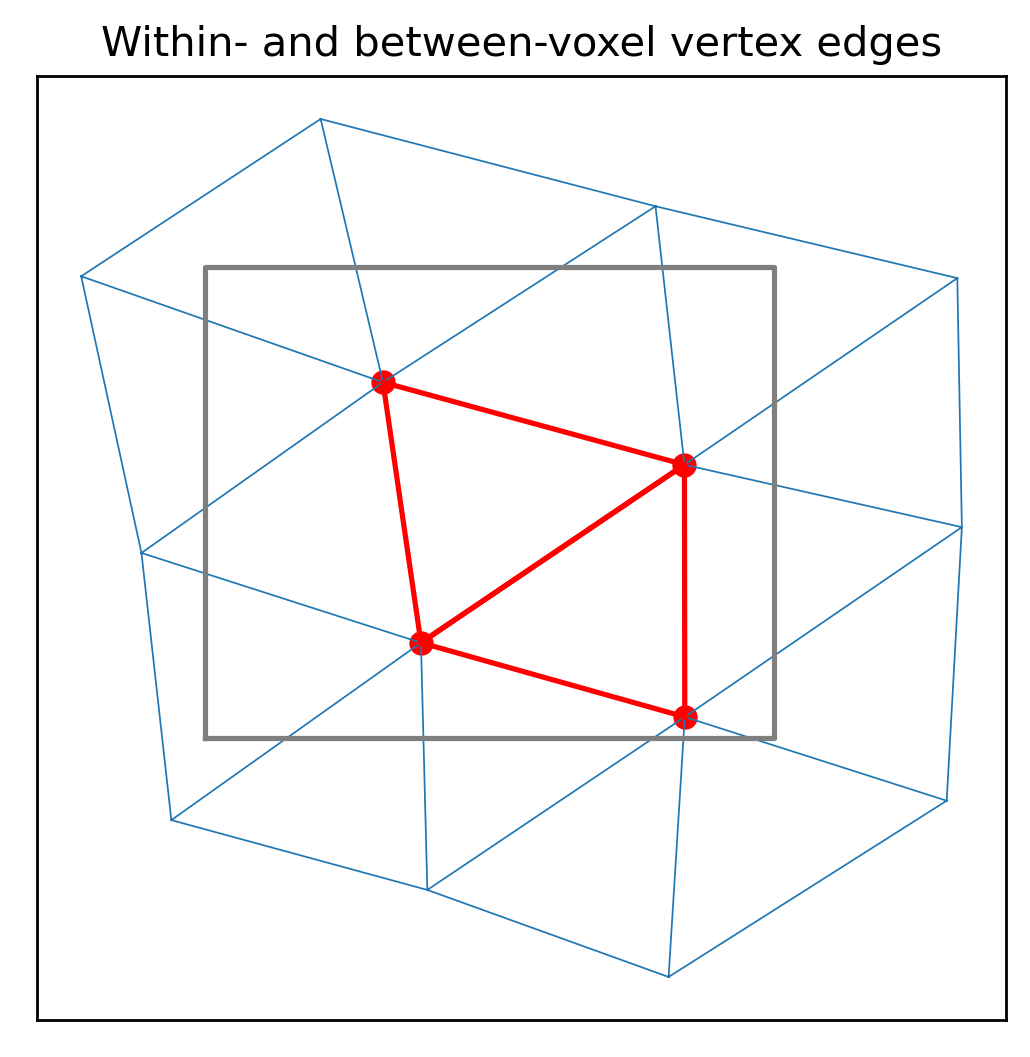
\includegraphics[width=0.6\textwidth]{disc_lap_edges.png}
\caption{Two-dimensional illustration of a cortical surface within a voxel. The vertices and edges that lie wholly within the voxel are coloured red, all other edges are blue. The principle of the discriminated Laplacian is that these edges should carry more weight because their connected vertices are in the same voxel. In contrast, difference is to be expected between voxels and therefore those edges should carry less weight.}
\label{disc_lap_edges} 
\end{figure}

In light of this, one can consider the existence of two related but distinct spatial priors. Firstly, a prior that applies between vertices contained in the \textit{same} voxel. It is expected that these should take very similar values as the resolution of the  data is not sufficient to support any other outcome (we cannot fit the data with sub-voxel resolution). Secondly, a prior that applies between vertices contained in \textit{different} voxels. It is expected that these will take somewhat similar values, and the resolution of the data is sufficient to support such an outcome: the vertices are in different voxels, so they are fitted to different data. 

The volumetric spatial prior implemented in FABBER can be considered as a special case of these two general priors: because all node connections are between-voxels as opposed to within, the former prior can be discounted entirely and only the latter holds. In contrast, in the surface case it has been observed that applying both priors with equal weight leads to suboptimal outcomes. The problem arises because the mesh Laplacian matrix does not distinguish between within-voxel connections (high similarity) and between-voxel (low similarity). It is hypothesised that this causes the optimisation to prefer excessively high values of $\phi$, for which it finds support from the numerous within-voxel connections that are fundamentally smooth to begin with, to the detriment of excessively smoothing across between-voxel connections. 

The solution that has been adopted is to discriminate between the two different types of connections, as illustrated in figure \ref{disc_lap_edges}. In particular, by assigning an extra multiplicative weight $\beta$ to within-voxel connections, they account for a greater overall contribution to the latent cost of the spatial prior and hence experience an increase in effective smoothing for the same value of $\phi$. Alternatively, one can regard the value of $\beta$ as reflecting a stronger belief in similarity for these connections. In either case, the resultant matrix may be considered as representing the union of two separate and distinct priors within a single operator. The construction of this matrix remains the same as for the mesh Laplacian with inverse distance weighting $n =$ 1, with the extra step that edges within the same voxel are multiplied by $\beta$. With $\beta = 1$ the conventional mesh Laplacian is recovered. The various forms of Laplacian discussed here are summarised in table \ref{laplacian_table}. 

\begin{table}[h]
\centering
\def\arraystretch{1.5}
\begin{tabular}{p{3cm}|p{11cm}}
\textit{name} & \textit{meaning}                                                                                                                                             \\ \hline
mesh          & Inverse distance weighting to neighbours                                                                                                                     \\
discriminated & Inverse distance weighting, with extra multiplicative weight $\beta$ on within-voxel connections. For $\beta$ = 1, this is equivalent to the mesh Laplacian.
\\
split         & Separate Laplacians for surface and volume spaces, with separate $\phi$ values                                                                               \\
joint         & Block diagonal concatenation of surface and volumetric Laplacians with single $\phi$ value                                                                   
\end{tabular}
\caption{Summary of different variants of the Laplacian matrix in surface and hybrid space.}
\label{laplacian_table}
\end{table}

It is possible to draw a comparison between this and the HCP approach to surface analysis of volumetric data. The same fundamental challenges of under-determinacy remain, though to a lesser extent (the resolution of HCP BOLD data is 2mm isotropic, which means there will be fewer surface vertices per voxel). The bigger difference between the methods, however, is that the HCP uses a purely analytic method to perform the \textit{forward} projection (volume to surface), whereas hybrid SVB uses the \textit{reverse} projection (surface to volume) as part of the inference. The forward projection used by the HCP is exactly determined: the value of any surface vertex is computed as an average of its surrounding voxels, weighted according to geometric quantities that are calculated independently of the data. All further analysis is then performed on the surface, without recourse to the volumetric space, so the challenge of under-determinacy does not arise: from the point of view of surface analysis, the data already exists in the same space as the analysis space thanks to the initial forward projection step. The penalty paid for this convenience is a reduction in the effective resolution of the data due to the averaging performed by the projection. These conditions do not hold true for surface SVB: the space of inference is \textit{not} the same as the data space, hence the under-determinacy of inference whereby multiple nodes are fitted to a single voxel remains a challenge. 

\section{Inclusion of acquisition noise}

The final change to volumetric SVB that was necessary to enable surface inference concerns the inclusion of acquisition noise within the generative model. A key attribute of VB is that allows for a principled treatment of noise that is specific to the system under investigation. The distributional properties of noise are therefore included as another parameter to be estimated alongside physiological parameters (in the case of ASL, a Gaussian distribution of zero mean and some variance). Under hybrid inference, this must be caveated: though it is possible to conceptualise physiological parameters existing `on the surface' or `in the volume', theoretical understanding of noise implies that it arises only in the volumetric space. This is because it is a consequence of the data acquisition process which is itself is volumetric. In practical terms, this means that noise is accounted for in volume space after model reconstruction: starting from a set of node-wise parameter estimates, model evaluation followed by projection into volume space yields a reconstruction of the data against which noise properties may be estimated. 

\section{Calibration of the spatial prior}
\label{prior_calibration}

In the course of development, it was observed that SVB applied a different level of smoothing to ASL data than would be obtained with FABBER. In order to further investigate these differences and determine a reasonable set of smoothing parameters, a series of calibration experiments were performed. This motivation should be considered in light of Penny \textit{et al.}'s statement in their earlier work on the spatial prior: ``as we gather more experience applying [the spatial prior] to fMRI data, we envisage, in the future, choosing $q_1$ and $q_2$ to reflect this knowledge" \cite{Penny2005}. 

\subsection{Datasets}

ASL data was simulated using similar parameters as in section \ref{pvec_simulation_data_section}, namely: pCASL of 1.8s label duration, 6 PLDs of 0.75, 1.0, 1.25, 1.5, 1.75, 2.0s with 4 repeats at each PLD. Three variants of data were used to investigate different scenarios. Structural pre-processed data, including cortical surface reconstructions, from subject 103818 of the HCP were used to define subject anatomy. 

\subsubsection{Volumetric smoothing}

The following two datasets were used to investigate the performance of the spatial prior in the volumetric space. Under SVB, only WM parameters are estimated in volume space and so the analysis was restricted to this tissue only.  

To simulate the impact of acquisition noise, data was simulated with constant parameter values of 60, 20 \cbf of CBF and 1.3, 1.6s ATT in GM and WM respectively. Using the definition of SNR established earlier in equation \ref{snr_defn}, SNR was set at 27, a favourable level compared to the representative level of 9 previously established. In the ideal case, SVB would smooth over the noise in the data and return low variance parameter estimates.

To simulate the impact of variance in parameters, data was simulated with parameters drawn from normal distributions. For CBF, these were $N(60,\ 8^2)$ and $N(20,\ 3^2)$ \cbf; for ATT $N(1.3,\ 0.15^2)$ and $N(1.6,\ 0.25^2)$ s; for GM and WM respectively. Low levels of noise were added to the data to yield an SNR of 90. Superficially, this dataset is similar to the acquisition noise case (there is significant variation in signal values between neighbouring voxels at any point in time) but mathematically they are quite different: in the former case, the variation is without meaning, whereas in the latter case the variation is meaningful as it is driven by underlying parameter variation. Equivalently, variation between voxels in the former case can be considered as noise of low bias and high variance, whereas in the latter it can be considered as noise of high bias and low variance. In the ideal case, SVB would not smooth over this variation between voxels and return variable parameter maps.

\subsubsection{Surface smoothing}

To investigate the performance of the spatial prior on the surface, a single dataset simulating areas of hypo- and hyper-perfusion was produced. The particular focus for this experiment was on the preservation of spatial detail on the cortical surface and as such the analysis considered cortical GM CBF only. Data was produced by evaluating a sinusoidally varying field of 60 \cbf\ CBF with maximum variation of $\pm$ 25 and then interpolating these values onto the inflated cortical surface. All other physiological parameters were held constant with the same values as in the acquisition noise dataset and SNR was set at 18. The ground truth CBF map on the surface is illustrated in figure \ref{lap_comparison}. In the ideal case, SVB would preserve the detail of the activation map on the surface and not apply excessive smoothing. 

\subsection{Methods}

All data was processed using hybrid SVB with the learning rate held constant at 0.5 for 750 epochs. Five gradient samples were taken at each optimisation step and the batch size was equal to the number of PLDs. Values of $q_2$ and $\beta$ = 1, 10, 100, 1000 were investigated (where $\beta$ implies the discriminated Laplacian), as was the joint Laplacian (a concatenation of the standard Laplacians in each space). 

For a comparison of smoothing in the volumetric space only, BASIL was used as a comparator method operating in PVEc mode. The spatial prior was enabled on GM and WM CBF but not ATT, which is default behaviour. For PVEc, BASIL uses a two-step approach that first fits a single-tissue model to all voxels, which is used as an initialisation for a two-tissue fit in GM and WM separately. By contrast, hybrid inference directly estimates GM and WM parameters without initialisation. 

\subsection{Results}

\begin{figure}[H]
\centering
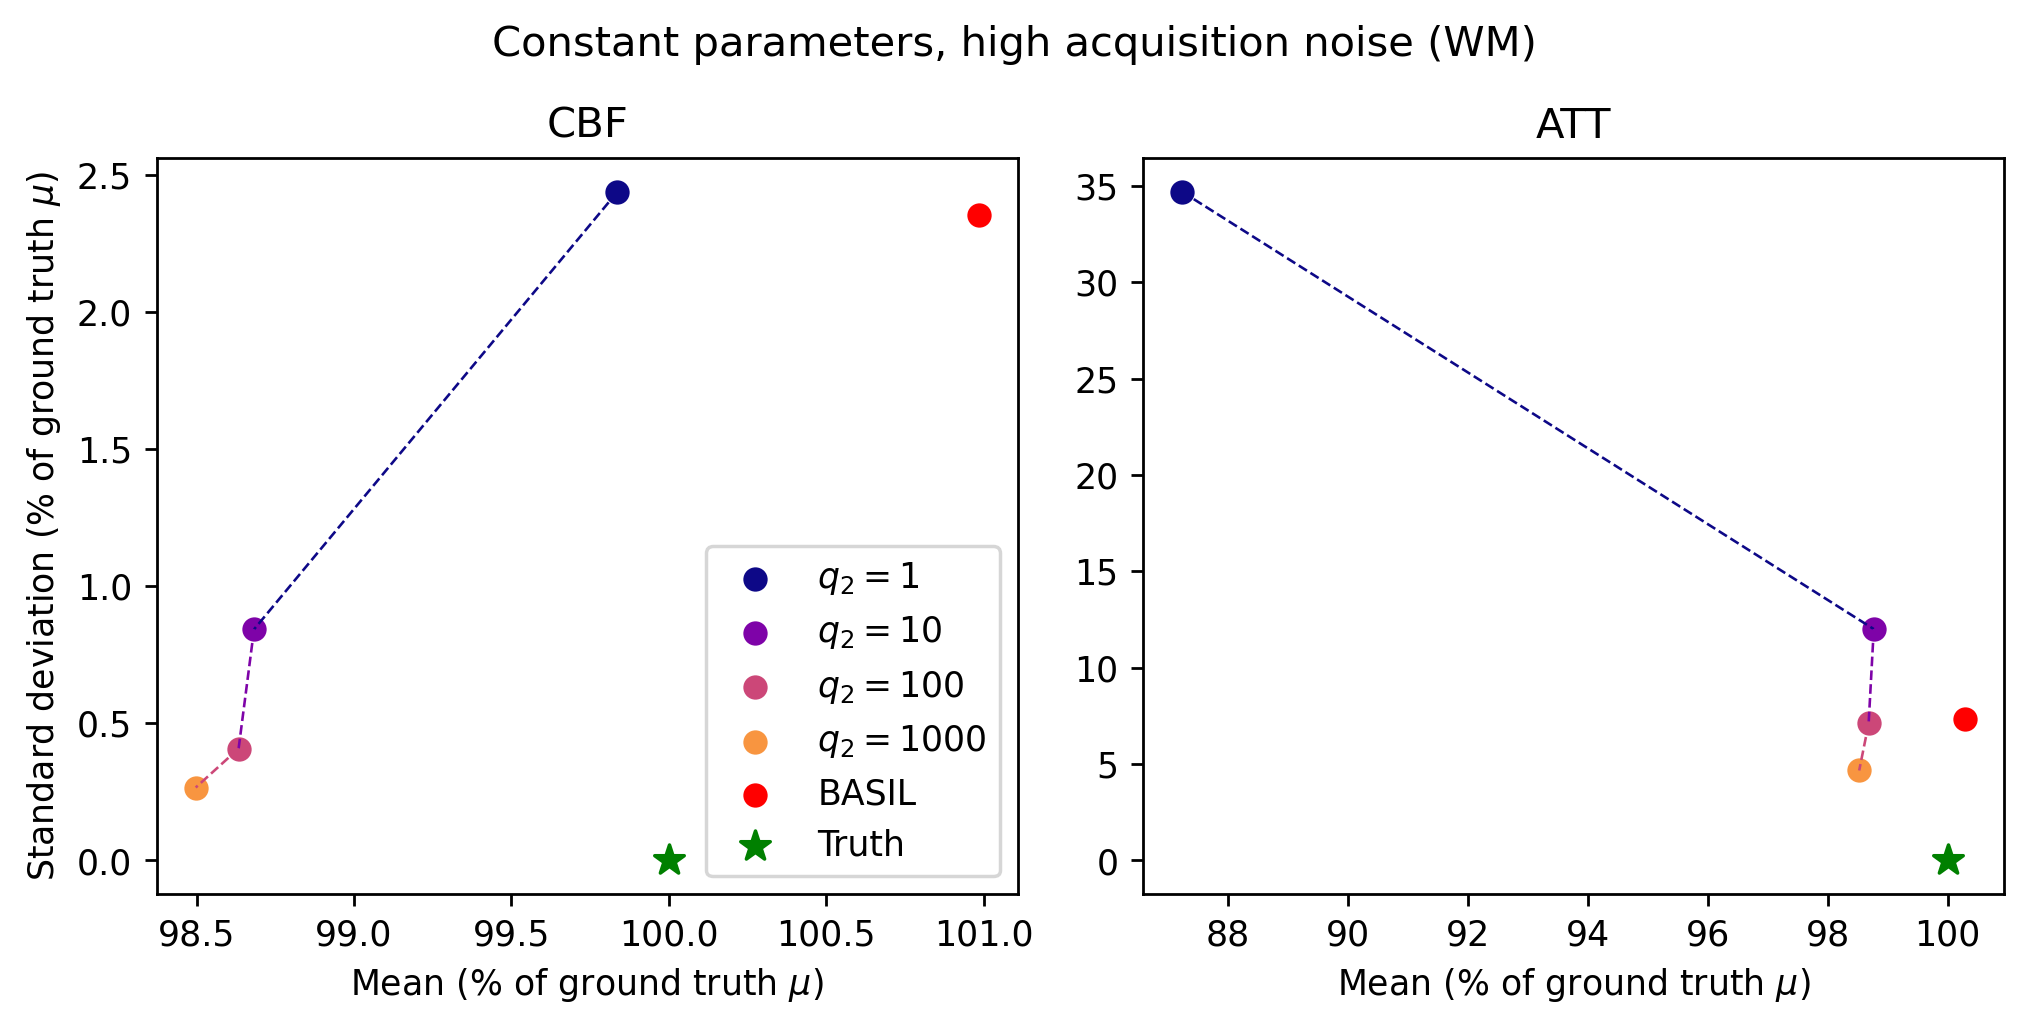
\includegraphics[width=\textwidth]{acquisition_noise.png}
\caption{Volumetric smoothing in the presence of high acquisition noise. Left: for CBF, varying $q_2$ levels demonstrated a trade-off in bias and variance, values of 10-100 were closest to ground truth. BASIL displayed low bias but higher variance. Right: for ATT, the lowest value of $q_2$ resulted in significant negative bias; values around 10-100 gave results closer to ground truth and to those of BASIL.}
\label{acquisition_noise} 
\end{figure}

Figure \ref{acquisition_noise} shows the effect of the volumetric spatial prior in the presence of high acquisition noise. In CBF, varying $q_2$ revealed a trade-off between bias and variance; high values resulted in lower variance but positive bias. BASIL demonstrated low bias but higher variance. In ATT, $q_2$ = 1 resulted in substantial negative bias, demonstrating that at least a small amount of smoothing was important for successful recovery of ground truth. Across both parameters, values of $q_2$ = 10-100 gave the best performance. 

\begin{figure}[H]
\centering
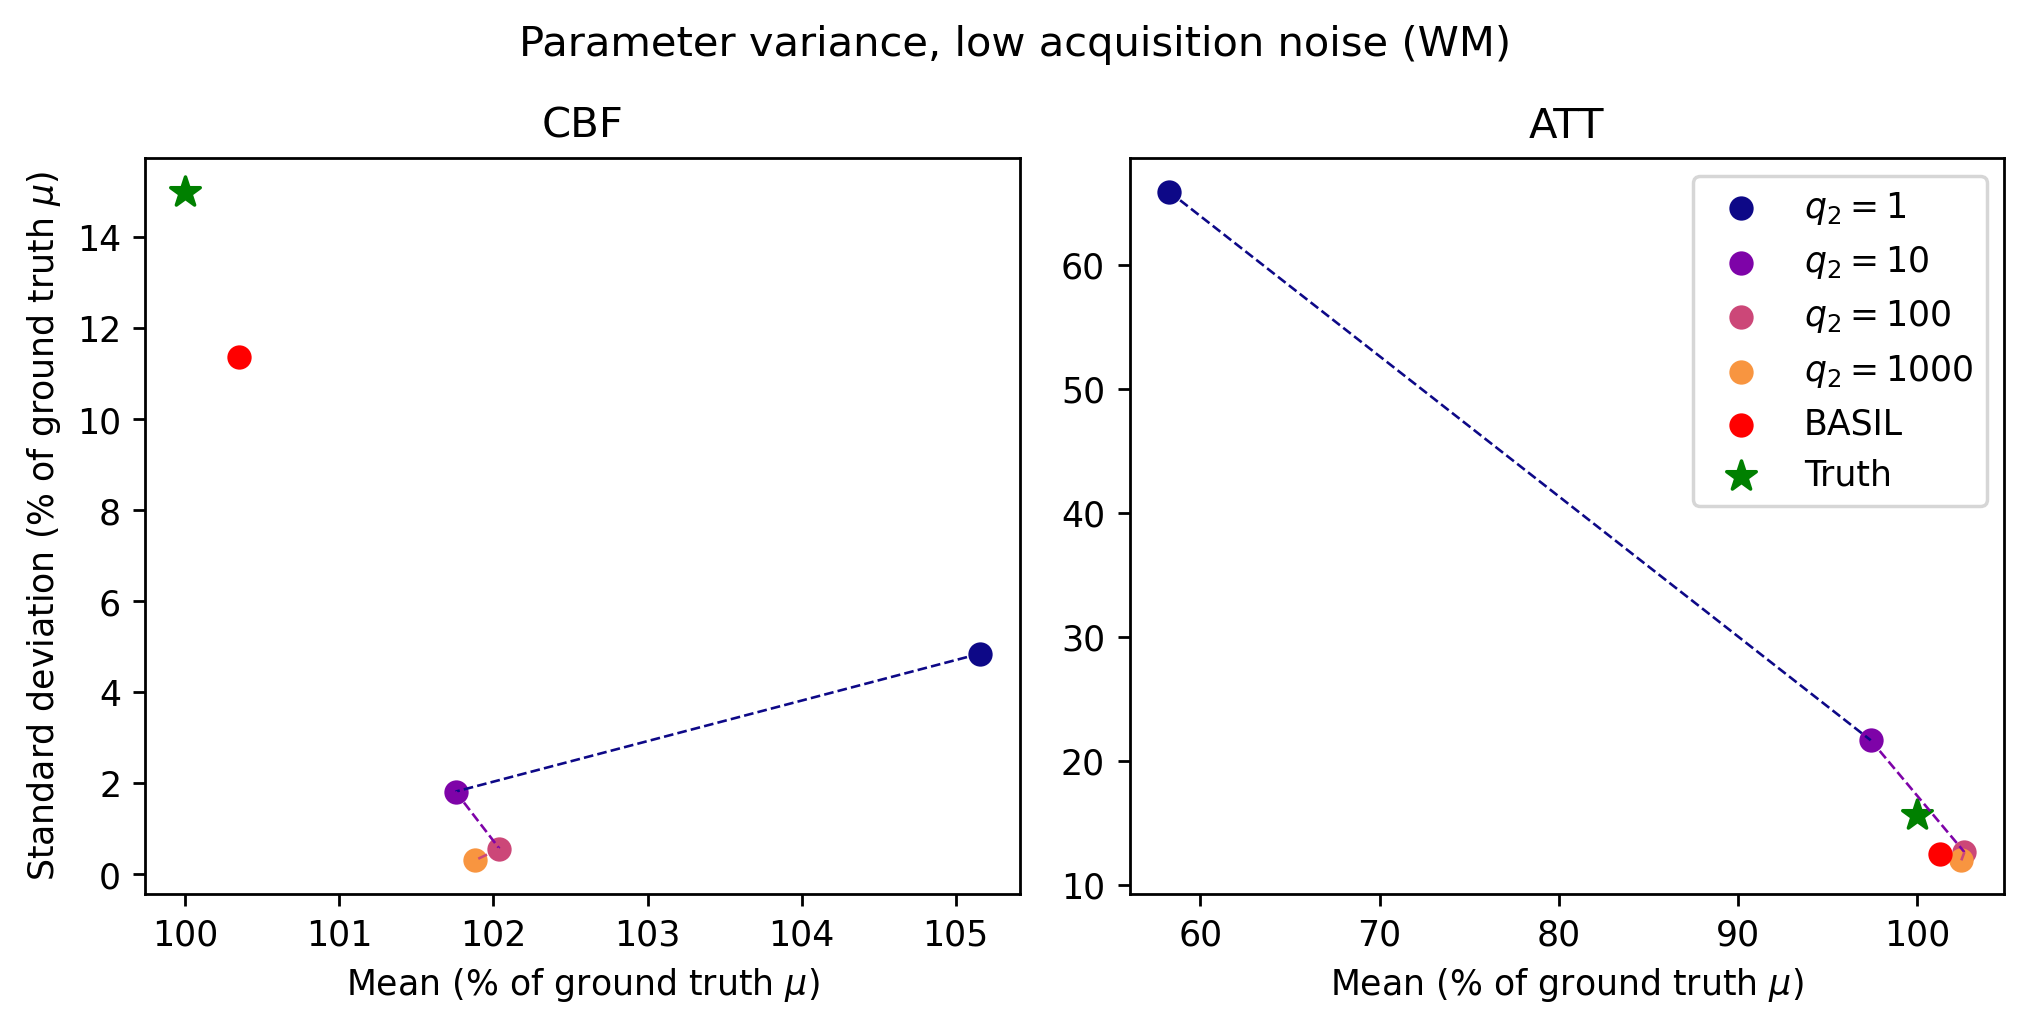
\includegraphics[width=\textwidth]{parameter_noise.png}
\caption{Volumetric smoothing in the presence of parameter variation. Left: for CBF, all values of $q_2$ resulted in excessively low variance compared to ground truth, though higher values also resulted in a smaller bias. BASIL was much closer to ground truth. Right: for ATT, higher values of $q_2 >$ 10 significantly improved recovery of ground truth, and values closer to BASIL.}
\label{parameter_noise} 
\end{figure}

Figure \ref{parameter_noise} shows the effect of the volumetric spatial prior in the presence of parameter variation. In CBF, all values of $q_2$ led to excessively low variance compared to ground truth, though increased values did also reduce bias. In ATT, higher values of $q_2$ led to much better recovery of ground truth. BASIL performed extremely well in relative terms for both CBF and ATT. Across both parameters, values of $q_2$ = 10-100 again gave the best performance. 

\begin{figure}[H]
\centering
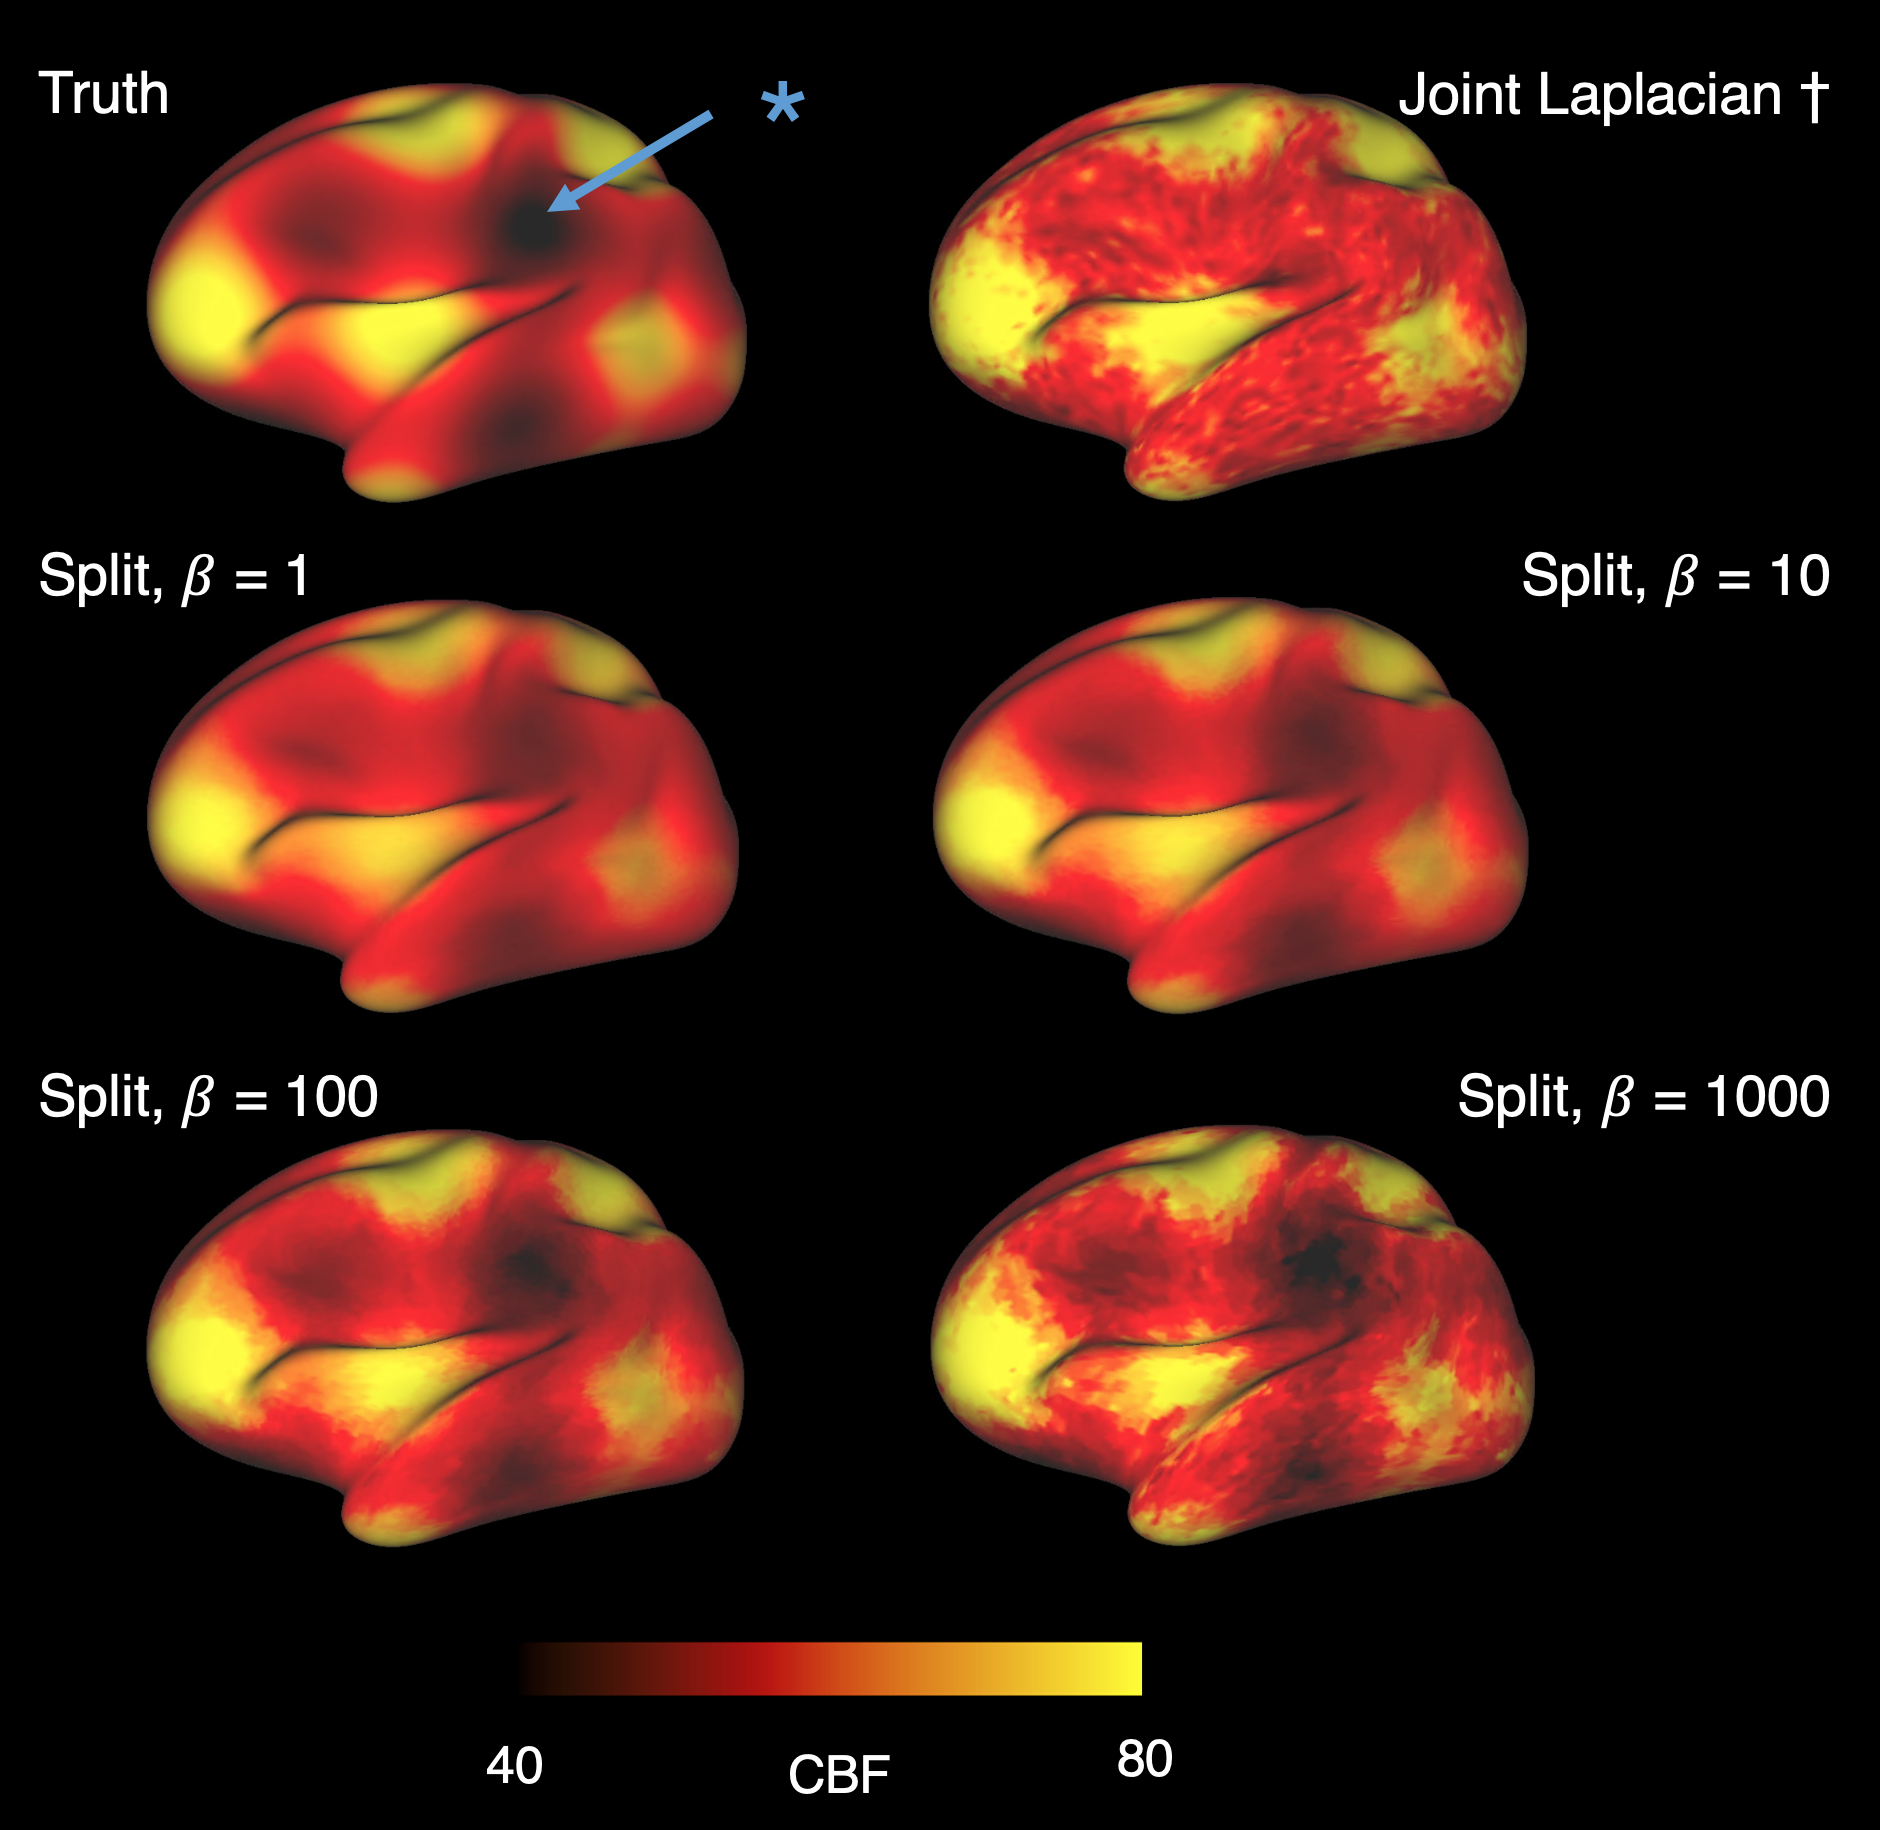
\includegraphics[width=\textwidth]{lap_comparison.png}
\caption{Surface smoothing under different formulations of the Laplacian. The true CBF map is shown top left, the blue star denotes an area of substantial hypo-perfusion. The joint Laplacian returned a CBF map that correctly preserved relative differences between high and low areas, but with a substantial positive bias, resulting in the elimination of all areas of hypo-perfusion and peak values 20\% greater than ground truth. †[The fit in WM was also extremely poor in this case, returning negative values in both CBF and ATT.] Various formulations of the split and discriminated Laplacian showed a good ability to preserve relative differences on the surface without introducing as great a bias; $\beta$ = 100 was empirically determined to offer the best compromise.}
\label{lap_comparison} 
\end{figure}

Figure \ref{lap_comparison} shows the effect of the surface spatial prior under different formulations of the Laplacian. Although the joint Laplacian returned a map that superficially preserved the relative differences between areas of hyper- and hypo-perfusion, there was also substantial positive bias that resulted in the elimination of all areas of hypo-perfusion in absolute terms. All formulations of the split and discriminated Laplacian showed the ability to preserve detail without introducing as severe a bias; $\beta$ = 100 was empirically determined to offer the best trade-off between preserving ground detail and rejecting noise. 

\subsection{Discussion}

In the volumetric space, SVB was observed to produce CBF estimates of much lower variance than the corresponding ATT estimates (standard deviation of around 1-5\% of baseline for CBF, versus 10-20\% for ATT). For ATT, a relationship between $q_2$ and mean estimate (\textit{i.e.}, bias in the estimates) was observed: in both the acquisition noise and parameter variance scenarios, values of $q_2 <$ 10 yielded mean ATT estimates substantially below ground truth. This behaviour was also observed to a lesser extent on CBF. Such a result indicates at least some amount of smoothing is required to attain a plausible fit, especially in ATT. This may in part be related to the challenges of estimating WM parameter values for ASL data. With a notably lower CBF and longer ATT, the SNR in WM is reduced compared to that of GM, which presents a challenge for parameter estimation. On the basis of these results, a value of 100 for $q_2$ was deemed to be optimal for the analysis of representative ASL data and all further work was performed using this value. 

In general, BASIL returned estimates closer to the ground truth value, with the exception of standard deviation of CBF in the acquisition noise scenario, which was somewhat higher than ground truth. Nevertheless, the contrast in BASIL's CBF estimates between the acquisition noise and parameter variance scenarios was clear: standard deviation in the former was notably lower than it was in the latter, which is the ideal outcome of \textit{data-driven} smoothing. It should also be noted that BASIL did not use a spatial prior on ATT whereas SVB did. This is default behaviour for BASIL and a normal distribution prior centred on 1.6s was instead used. BASIL yielded around 10\% standard deviation in ATT on \textit{both} the acquisition noise and parameter variance datasets, which suggests that the variability of estimates produced was more a function of the distributional prior than of the data itself, \textit{i.e.}, somewhat less data-driven. 

Estimating ATT via hybrid SVB using the same normal distribution prior as for BASIL was investigated but discounted due to poor performance. This was because, in the presence of high acquisition noise, negative ATT values were occasionally returned. Inferring the logarithm of ATT (a restriction to positive values) was also investigated, but this merely treated the symptom of the problem rather than the cause: a tendency towards negligibly small ATT, which corresponds to very low signal being present in the voxel at later PLDs. In contrast, BASIL did not demonstrate this behaviour which suggests that the normal prior is more effective in constraining that inference than it is for SVB. This is a notable point of divergence between volumetric SVB and BASIL, and, given that their performance in this space should be approximately equivalent, merits further investigation. 

In surface space, the different formulations of Laplacian were observed to have a substantial impact on the mean and spatial distribution of the parameter estimates returned. Starting with the base case of the joint Laplacian covering both the surface and volumetric spaces, the large positive bias in estimates (particularly evident in areas of hypo-perfusion) was deemed too problematic for continued use. The joint Laplacian also resulted in extremely poor performance in the WM space, which, as the volumetric results show, required a minimum level of smoothing to obtain plausible estimates. 

In contrast, all variants of the split and discriminated Laplacian allowed for the preservation of spatial detail without the substantial positive bias demonstrated by the joint form. With $\beta$ = 1 (no difference in within- and between-voxel weighting), the conventional distance-weighted mesh Laplacian was recovered and this yielded a desirably smooth map, though the CBF range (difference between maximum and minimum) was substantially reduced compared to the ground truth. Increasing values of $\beta$ yielded improvements in range, particularly in respect of preserving areas of hypo-perfusion. Accordingly, a value of $\beta$ = 100 was selected as giving optimal performance for the analysis of representative ASL data and used for all subsequent work presented herein. 

The poor performance of the joint Laplacian may be understood in terms of the two inference spaces requiring fundamentally different levels of smoothing in order to obtain optimal fits. Under the application of the joint Laplacian, the optimisation was forced to choose a single value of $\phi$ for both spaces. In the results presented here, the more optimal value for the surface was generally selected, resulting in poor WM performance, but sometimes the opposite outcome would be attained: an optimal smoothing value for volume space, which resulted in the near total elimination of detail on the surface (illustrated in figure \ref{smooth_surface}). Concerningly, this alternation in smoothing levels was a transient behvaiour that could not reliably be reproduced, further emphasising the challenges of using the joint Laplacian. 

\begin{figure}[H]
\centering
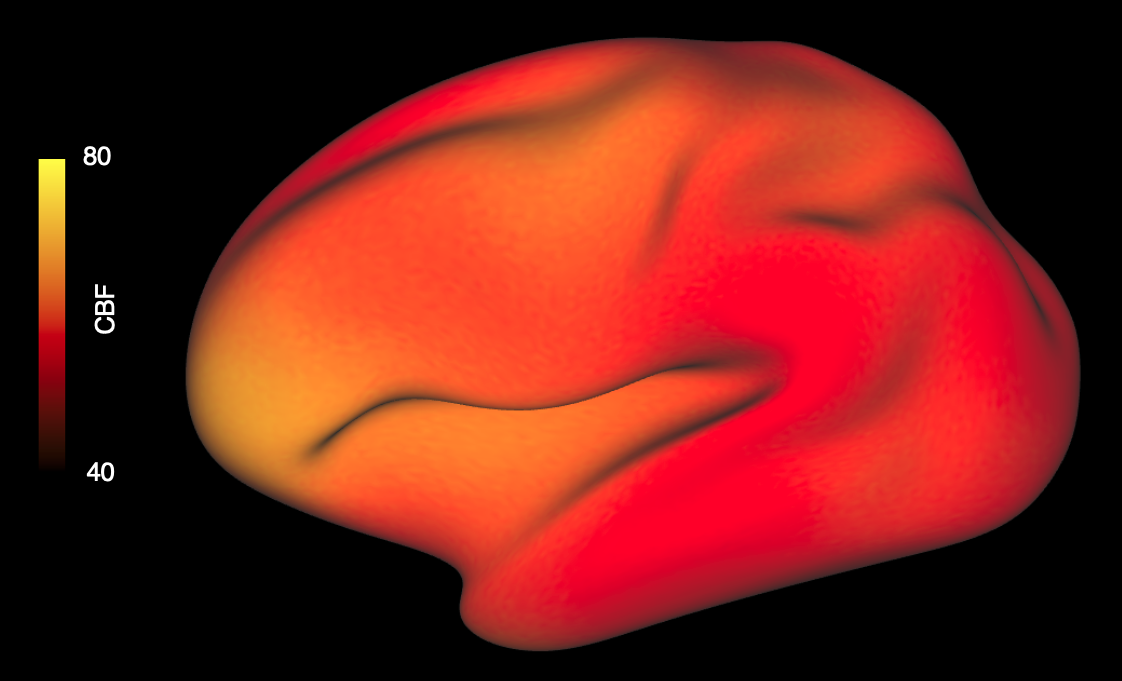
\includegraphics[width=0.8\textwidth]{smooth_surface.png}
\caption{Example cortical CBF estimates under application of the joint Laplacian, in a scenario where the amount of smoothing selected was more optimal for volume space. This resulted in the elimination of almost all detail on the surface.}
\label{smooth_surface} 
\end{figure}

By contrast, application of the prior separately to each space, with separate $\phi$ values, allowed a more optimal fit to be attained in both simultaneously. This is confirmed by the different values of $\phi$ selected during the course of optimisation that are illustrated in figure \ref{ak_values}: the value selected for volume space was an order of magnitude greater than that selected for the surface. 

\begin{figure}[H]
\centering
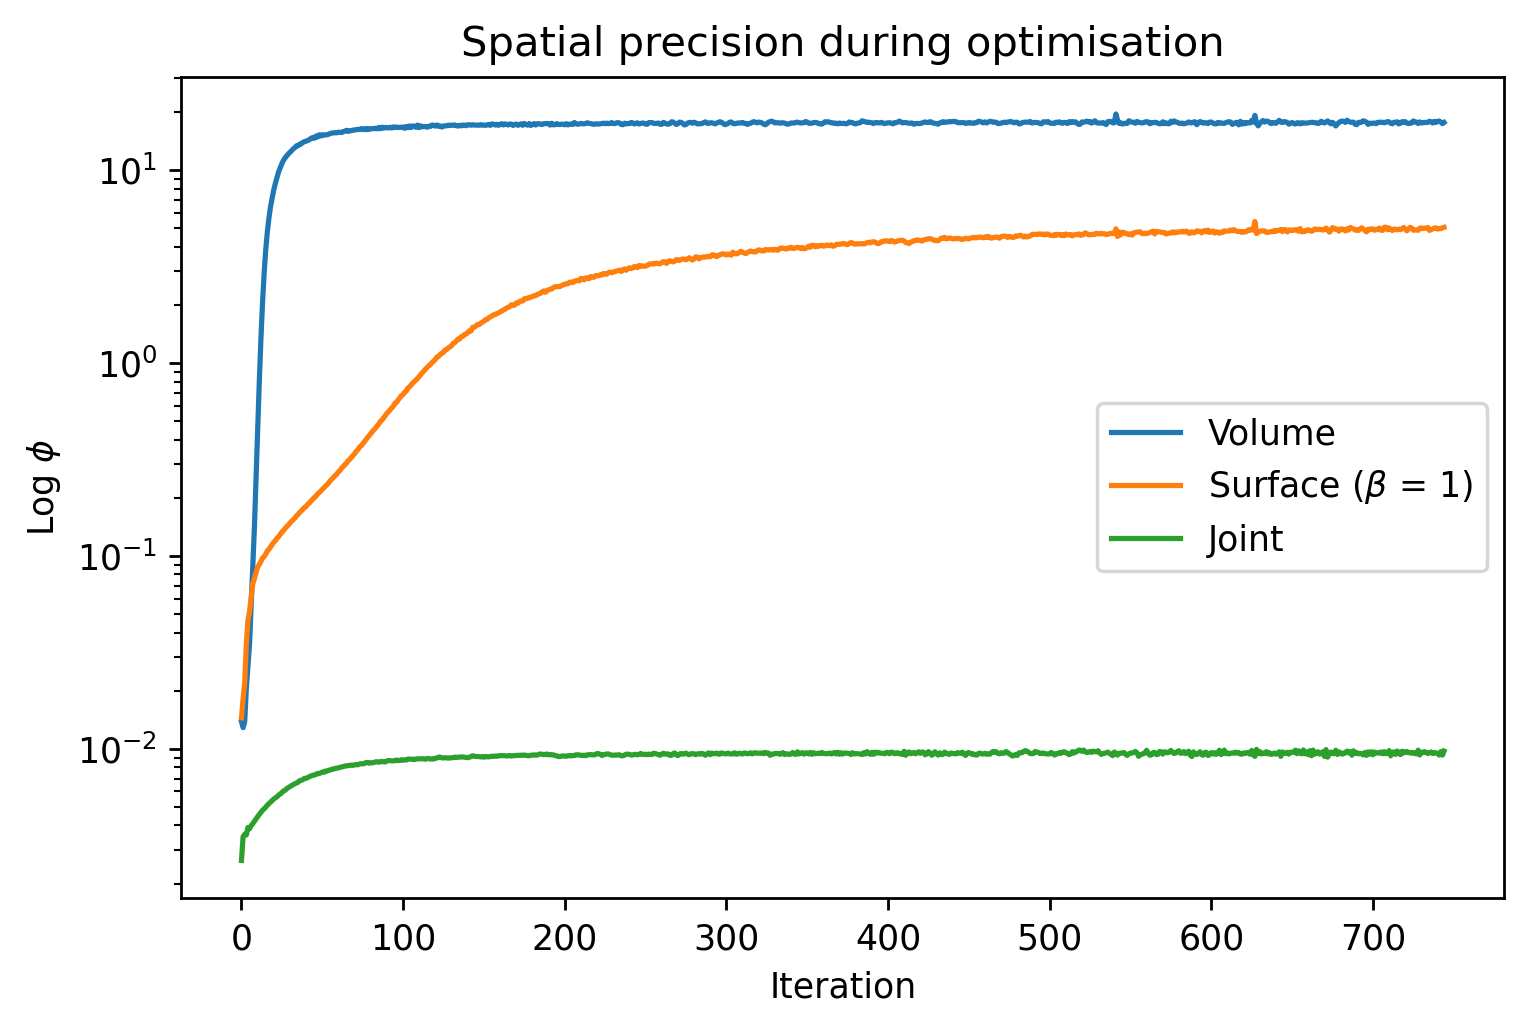
\includegraphics[width=0.75\textwidth]{ak_values.png}
\caption{Evolution of $\phi$ for the volumetric and surface spaces during optimisation, using a split but not discriminated Laplacian (\textit{i.e.}, $\beta$ = 1). The value in volume space was an order of magnitude higher than for surface space, demonstrating the fact that they require different levels of smoothing. By contrast, under the joint Laplacian $\phi$ was restricted to small values, suggestive of a local minimum in that parameter space.}
\label{ak_values} 
\end{figure}

There are many possible explanations as to why this difference arises. Firstly, it was observed for both BASIL and SVB that $\phi$ is not magnitude-invariant (its value varied inversely with the magnitude of the parameter to which it pertained). For example, PVEc under BASIL applies a volumetric spatial prior to both GM and WM CBF; the value of $\phi$ obtained for the former tissue was smaller than for the latter. As CBF values are expected to be higher in the cortex than for the subcortex, it is also expected that $\phi$ will be smaller. One implication of this is that the existing Gamma prior on $\phi$ used by BASIL may actually be effectively tighter for WM than it is for GM (because values of $\phi$ for WM will naturally be higher, and therefore closer to the edge of the distribution). 

Also as a result of this property, figure \ref{ak_values} reveals one of the drawbacks of using the discriminated Laplacian with parameter $\beta$: a substantially reduced value of $\phi$ for surface space. Because the discriminated Laplacian increases the weight associated with within-voxel connections, the SSD quantity $\frac{\phi}{2}\theta_i^T\mat{D}\theta_i$ is increased for a given $\theta_i$, which leads to smaller values of $\phi$ being selected. This renders the Gamma prior with $q_2$ = 10 or 100 on $\phi$ extremely uninformative: the value of $\phi$ is so small compared to the bounds of the distribution that the prior plays no role whatsoever. In effect, by using the discriminated Laplacian, one swaps control of smoothing in surface space via $q_2$ for control via $\beta$ (and, to boot, note that values of 100 were found to be approximately optimal for both of them). This merits further investigation. 

A second possible explanation is the differing magnitude of edge weights contained within the Laplacian matrix of each space. Under FABBER's existing framework, a Laplacian with unity edge weighting is used, but this was not carried over into SVB. This was partly to allow for better treatment of anisotropic voxel grids and partly to enable the creation of a joint Laplacian covering both the surface and volume spaces. On a 32k cortical surface, the mean distance between vertices (around 1mm) is much smaller than the mean distance between ASL voxel centres (around 3mm); it was therefore deemed appropriate to apply inverse distance weighting to the Laplacian so as to respect this difference in neighbour distances. The consequence of this, however, is to make the individual elements of the surface Laplacian larger than those of the volumetric, which therefore means the SSD quantity $\frac{\phi}{2}\theta_i^T\mat{D}\theta_i$ also becomes larger due to the linear scaling in $\mat{D}$. This means that for a given $\theta_i$, the same latent cost can be achieved with a smaller $\phi$. Note also that this mechanism explains why a calibration of the Gamma parameter $q_2$ for the volumetric space was necessary in the first place: compared to FABBER's unity edge weighting, SVB's volumetric Laplacian has much smaller elements (1/3 for a 3mm voxel grid). In order to obtain the same value of $\frac{\phi}{2}\theta_i^T\mat{D}\theta_i$ as for BASIL's Laplacian, the value of $\phi$ must \textit{increase} by a corresponding amount, but this is not possible unless the Gamma prior is relaxed, \textit{i.e.}, a higher value of $q_2$ is used. In this regard, the improved volumetric performance obtained with $q_2$ = 100 was entirely as expected. 

Finally, and most importantly in the context of physiological imaging, the difference in optimal smoothing levels may potentially be explained in terms of the different underlying physiology of the anatomies represented by the two spaces. Although such an argument cannot be justified using the simulations presented here (they are not claimed to be entirely realistic), it may be that the length scale of parameter variation in the two spaces is fundamentally different, and therefore they will always require different levels of smoothing. Allowing separate application of the spatial prior in both spaces allows for this difference to be respected. 

\section{Evaluation on ASL data}

Following calibration of the spatial prior, an evaluation of SVB hybrid inference was performed using representative ASL data. The particular focus was ability to resolve areas of hypo- and hyper-perfusion on the cortical surface, as such a surface-based analysis is a key motivation for the hybrid approach. 

\subsection{Datasets}

\subsubsection{Simulated ASL hyper/hypo-perfusion}

Simulated ASL data with areas of hyper- and hypo-perfusion on the cortical surface (distinct to the earlier case of sinusoidal variation) was produced using anatomical data from subject 103818 of the HCP. Four repeat ASL timeseries in differing alignments were generated. The ASL signal was generated in hybrid space (\textit{i.e.}, separate cortical and subcortical contributions) and then projected into volume space using Toblerone's framework. White Gaussian noise was added in volume space. ASL sequence parameters were the same as used in section \ref{pvec_chapter_sim_data}, namely: multi-PLD pCASL of 1.8s label duration; 6 PLDs of 0.75, 1.0, 1.25, 1.5, 1.75, 2.0s, and 8 repeats per PLD. Using the same definition of SNR as presented in equation \ref{snr_defn}, data was simulated with SNR levels of 9 (realistic) and 27 (favourable). Runtime on a desktop computer with 8 CPU cores at 2.6GHz was around 15 minutes per acquisition; this could likely be reduced by an order of magnitude using the GPU hardware for which TensorFlow is optimised. 

The cortex as a whole was assigned a constant CBF value of 60 \cbf. ROIs were then generated from seven bilateral seed points on both hemispheres, as illustrated in figure \ref{roi_cbf_truth}. Twelve rounds of dilation were applied to each seed point to identify the first order, second order, ... $n$\textsuperscript{th} order neighbours; the vertices in these neighbourhoods were assigned an intensity of $\pm25 \cdot (1 - (\frac{n-1}{12})^3)$ to produce a broad signal peak that decayed with radial distance. The end result of this process was a surface ground truth CBF map containing areas of hypo- and hyper-perfusion of maximal difference relative to baseline of $\pm$25 \cbf. 

\begin{figure}[H]
\centering
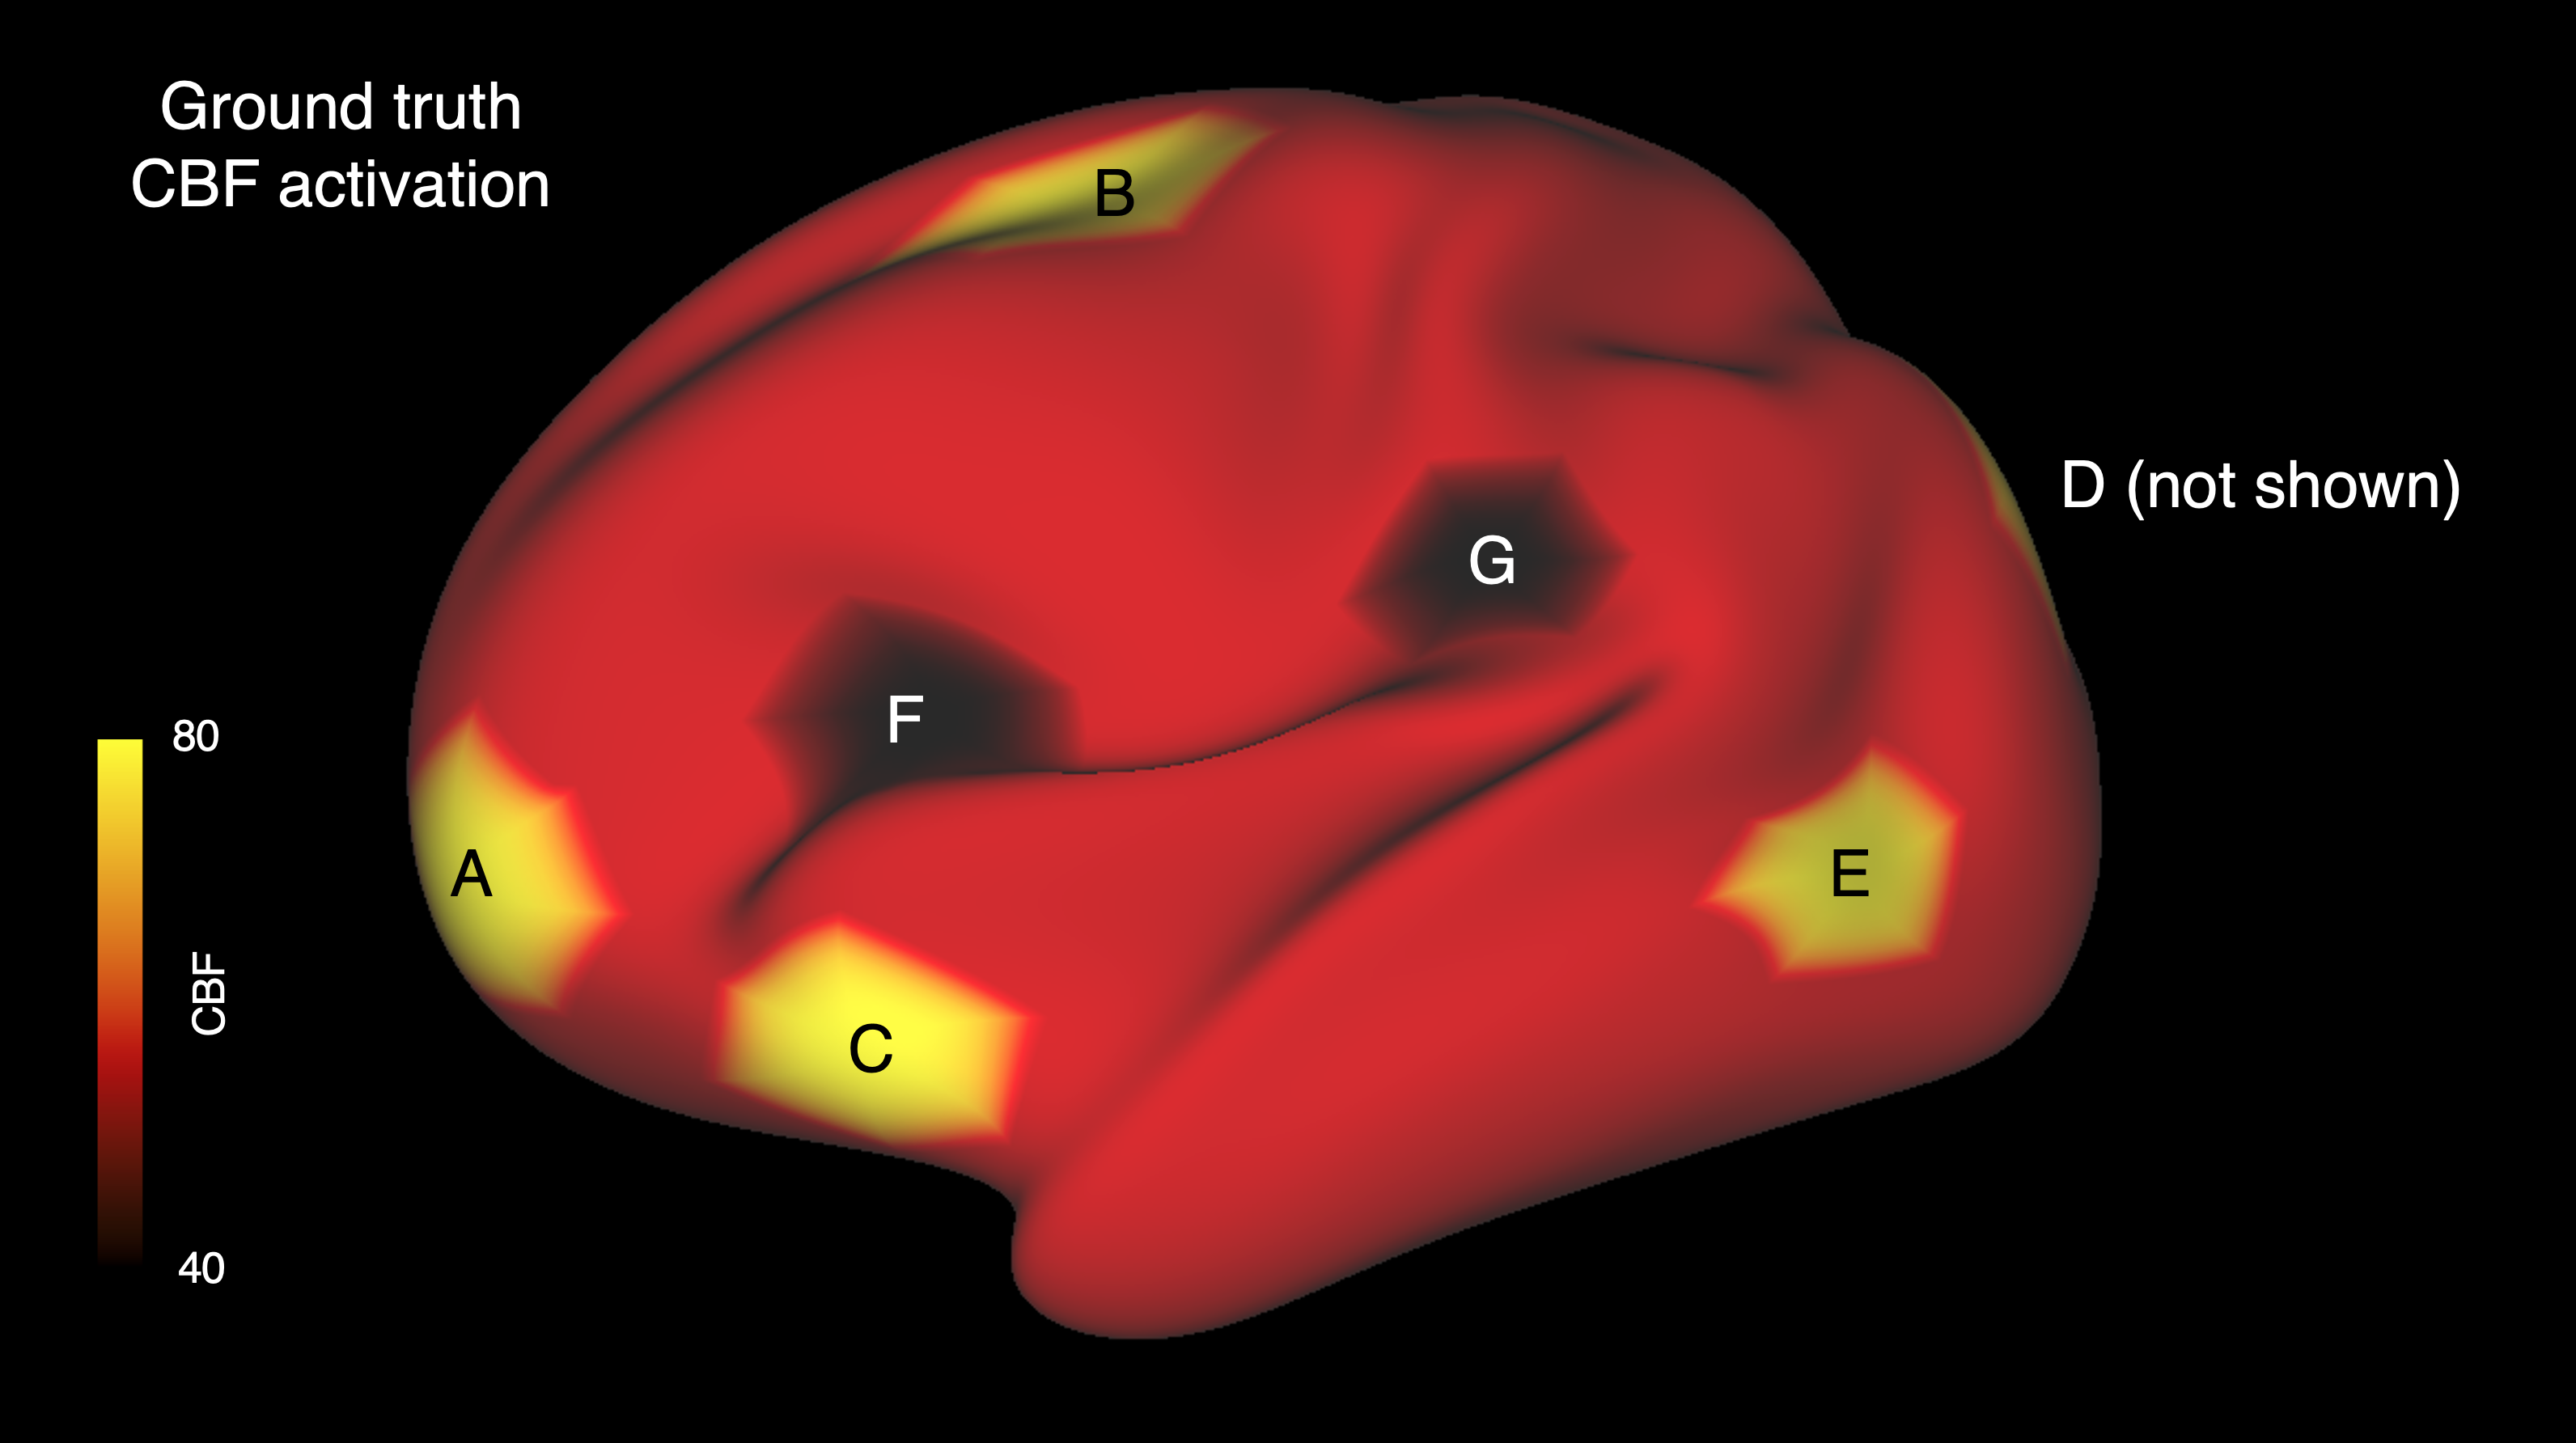
\includegraphics[width=\textwidth]{roi_cbf_truth.png}
\caption{Simulated areas of hypo-/hyper-perfusion on the cortex. Areas A - E have hyper-perfusion of +25 units; F and G have hypo-perfusion of -25 units. These areas were defined bilaterally on both hemispheres, though only the left is illustrated here.}
\label{roi_cbf_truth} 
\end{figure}


\subsection{Methods}

The data was analysed using the three strategies presented below, ranging from a fully surface-aware approach (SVB hybrid) to an entirely volumetric approach. 

\subsubsection{SVB hybrid}

SVB was run in hybrid mode to infer CBF and ATT for both cortical hemispheres and subcortical WM. For all runs, the learning rate was held constant at 0.5, five gradient samples were taken at each step, the data was divided into batches equal to the number PLDs, and fitting was run for 1000 epochs. Following the results of the spatial prior calibration, the $q_2$ scale term on the Gamma prior for spatial precision was set at 100, split spatial priors for the surface and volume spaces were used, and the discriminated Laplacian with $\beta =$ 100 was used for surface space. The spatial prior was enabled for both CBF and ATT. All estimation was performed in native acquisition space, resulting in surface parameter estimates that could be freely compared across repeats without registration (referring back to section \ref{tob_projector_paragraph}, the surfaces are registered to the data when initialising a Toblerone projector instead of the other way round). 

\subsubsection{BASIL projected}

This method comprises volumetric parameter estimation with PVEc followed by projection onto the cortical surface. BASIL was used for all analyses; Toblerone's volume to surface projection was used to project the PVEc GM CBF output maps onto the cortical surface. The spatial prior was enabled for CBF only (the default behaviour). All estimation was performed in native acquisition space and once again the surface parameter estimates could be compared across repeats without further registration. When comparing volumetric WM parameter estimates from this method, BASIL's output pre-projection was used and this variant is referred to as \textit{BASIL native} to emphasise the fact that no surface projection was required. 

\subsubsection{BASIL common}

This method represents an entirely volumetric analysis pipeline. The individual ASL repeats were transformed from their native alignments into common alignment, along with their corresponding PV estimates, using trilinear interpolation. All subsequent parameter estimation was performed in common space using BASIL, configured identically as for the BASIL projection method, and finally the results were left in common-aligned volumetric space. Although this meant that they were not directly comparable with the surface methods due to being in a different analysis space, this method was included to reflect the fact that volumetric analysis remains the dominant paradigm for ASL. 

\subsubsection{CBF analysis} 

CBF estimates produced by these methods were analysed in a number of different ways. Firstly, within ROIs, both the mean CBF and mean $Z$-score (number of standard deviations from the mean) were calculated. The latter was calculated across CBF estimates for the entire cortex and then the mean within each ROI extracted (when establishing mean CBF, no effort was made to exclude values from ROIs other than the one in question). The former metric gives an indication of absolute accuracy of CBF estimates within ROIs, whereas the latter gives an indication of relative differences between ROIs and baseline CBF. Finally, histograms of CBF estimates for the cortex and subcortex were used to evaluate distributional properties, in particular to investigate the presence of bias. 

In order to map the cortical ROIs into volume space for the analysis of BASIL common's results, binary masks representing the ROIs on the surface were projected using Toblerone's surface to volume projection. These were then thresholded to include only voxels for which each ROI contributed at least 75\% of the cortical PV (note that this is subtly different to saying that the voxel contains at least 75\% ROI PV; instead, of the voxel's cortical PV, at least 75\% of \textit{that} is within the ROI).

\subsection{Results}

\begin{figure}[H]
\centering
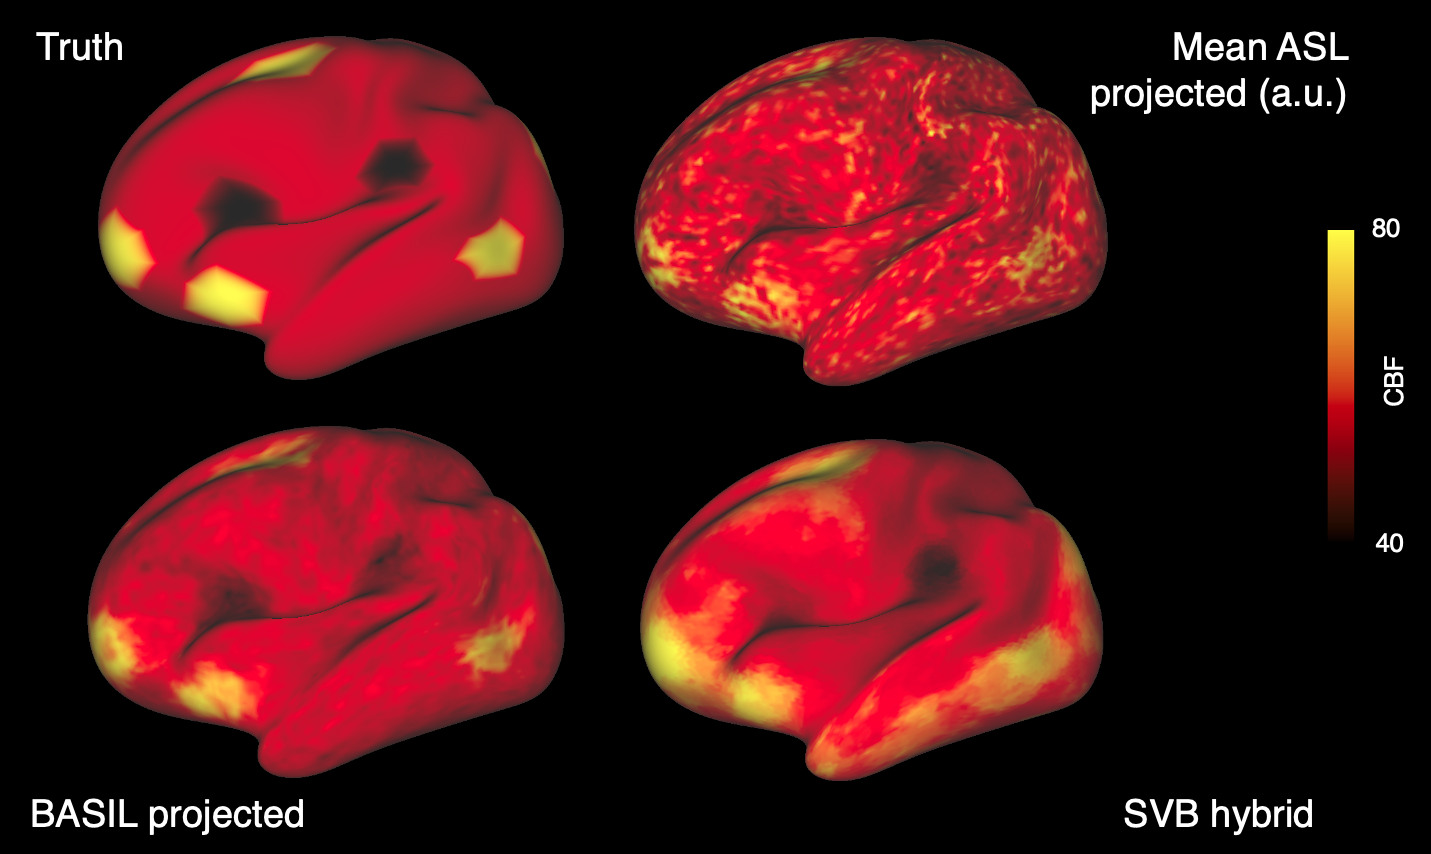
\includegraphics[width=\textwidth]{roi_cbf_comparison.png}
\caption{Cortical CBF maps, low SNR data. The timeseries-mean of the ASL data projected onto the surface demonstrates the substantial confound caused by high noise. In absolute terms, SVB hybrid was better able to recover the maximum signal values of ground truth than BASIL projected, though it also displayed positive bias in areas of hypo-perfusion where CBF was over-estimated. BASIL preserved the relative differences between ROIs, at the cost of reduced CBF range (difference between maximum and minimum).}
\label{roi_cbf_comparison} 
\end{figure}

Figure \ref{roi_cbf_comparison} shows estimated cortical CBF maps for a single repeat of the low SNR data. In absolute terms, SVB better reproduced areas of high perfusion, but did demonstrate some positive bias that led to over-estimation in areas of hypo-perfusion. BASIL projected was able to reproduce the relative differences between cortical areas, at the cost of a reduction in parameter range. Visually, the extent of smoothing appeared higher on the SVB estimates. 

\begin{figure}[H]
\centering
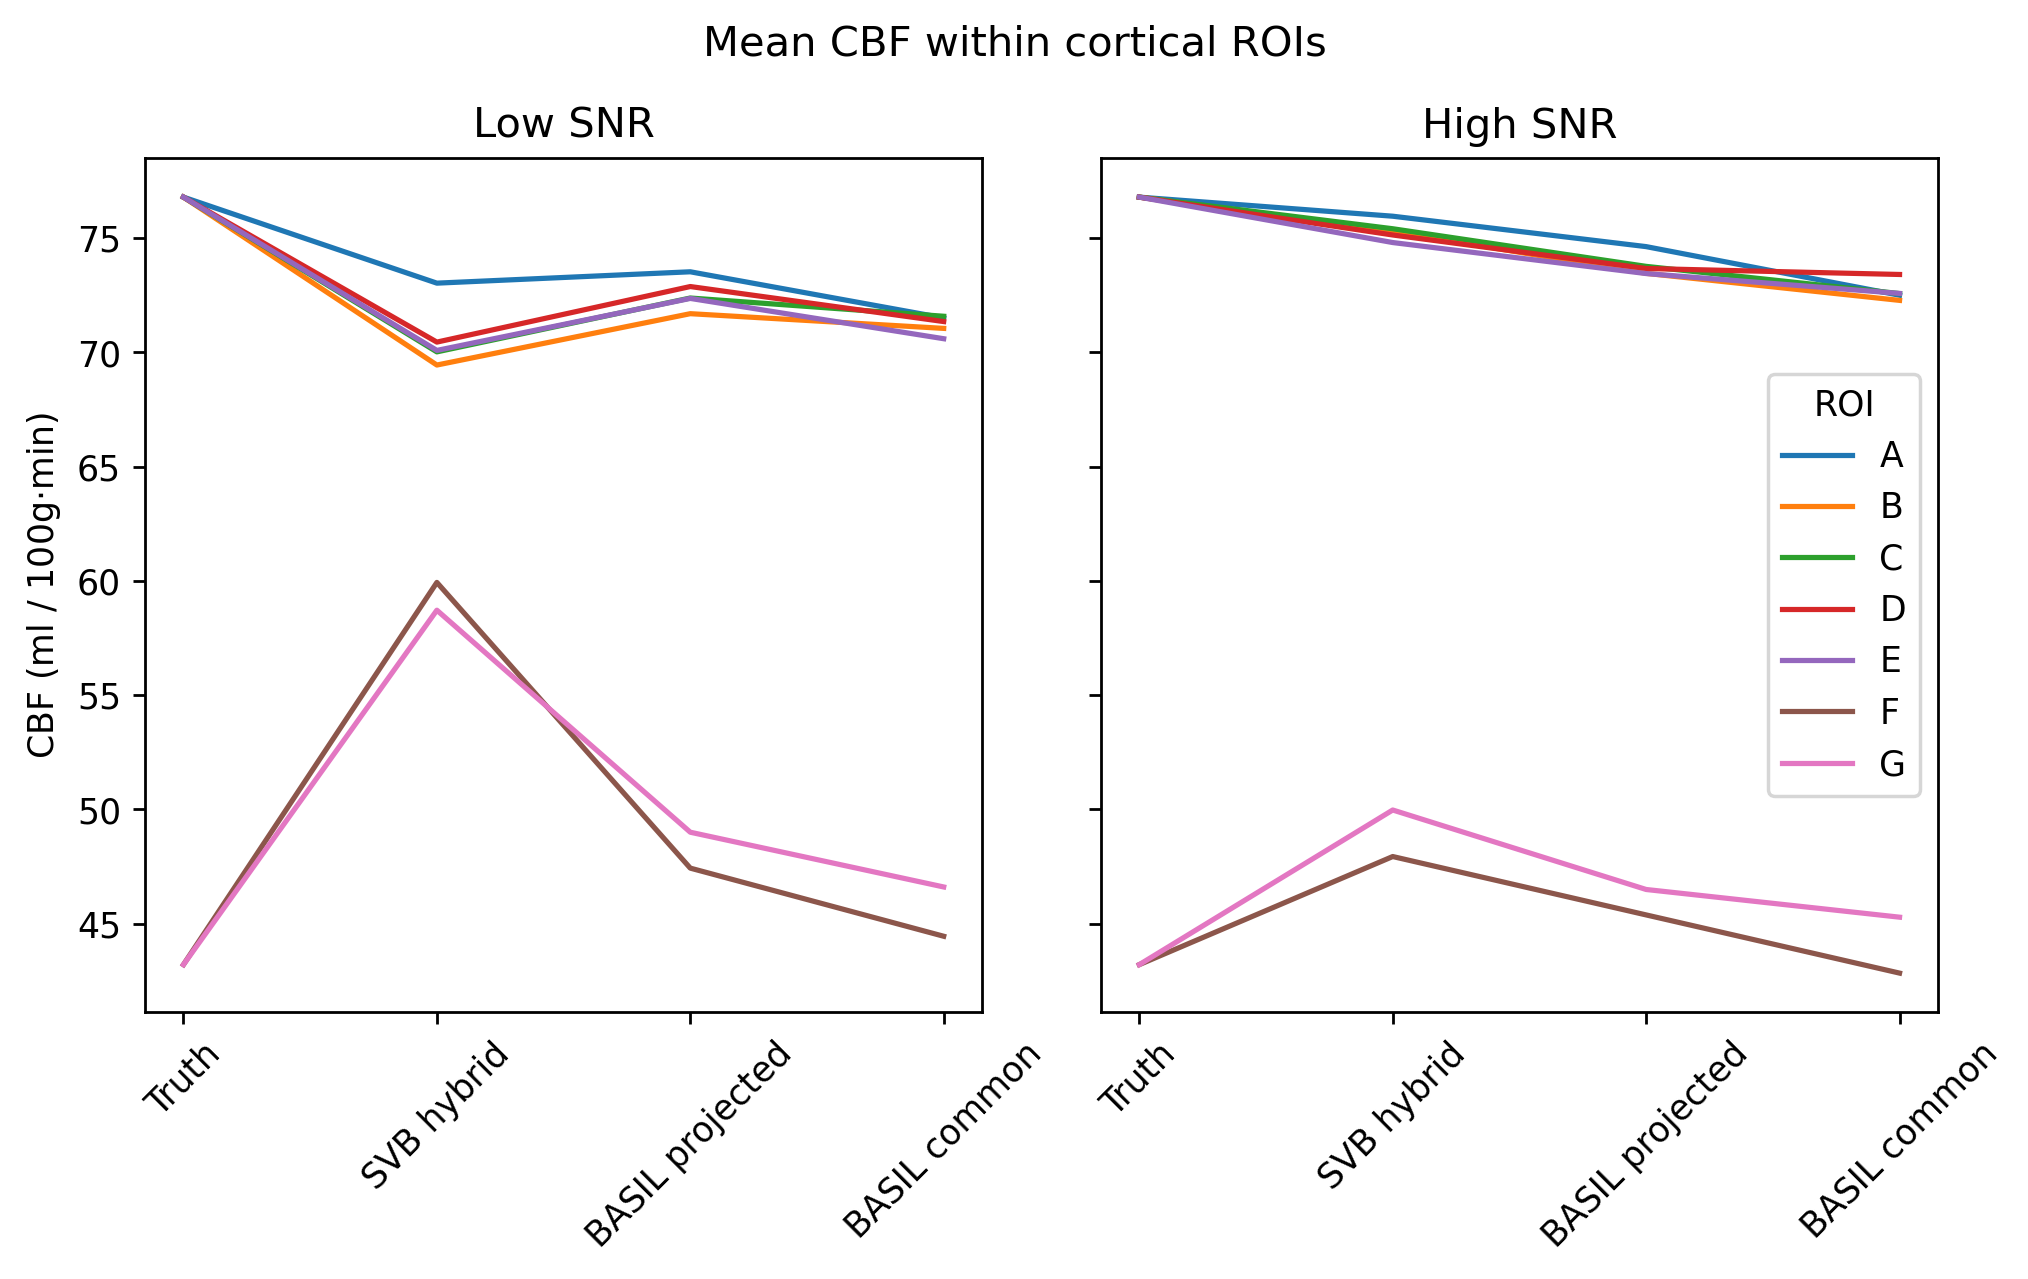
\includegraphics[width=\textwidth]{roi_cbf.png}
\caption{Mean CBF values within ROIs. With high SNR, SVB showed an excellent ability to estimate hyper-perfusion, though it struggled with low SNR. Further, there was a clear positive bias for areas of hypo-perfusion, sufficient to entirely eliminate these ROIs at low SNR. BASIL projected demonstrated good consistency at both noise levels. BASIL common was able to reproduce areas of hypo-perfusion but under-estimated areas of hyper-perfusion.}
\label{roi_cbf} 
\end{figure}

Figure \ref{roi_cbf} shows mean CBF within cortical ROIs. At high SNR, SVB was able to closely reproduce ground truth in areas of hyper-perfusion, though the presence of a positive bias for hypo-perfusion could clearly be seen. This was exacerbated in the low SNR data. BASIL projected demonstrated marginally higher errors relative to ground truth for both hyper- and hypo-perfusion, but, crucially, performance was relatively consistent at both noise levels. BASIL common was better able to estimate hypo-perfusion than hyper-perfusion at both noise levels. 

\begin{figure}[H]
\centering
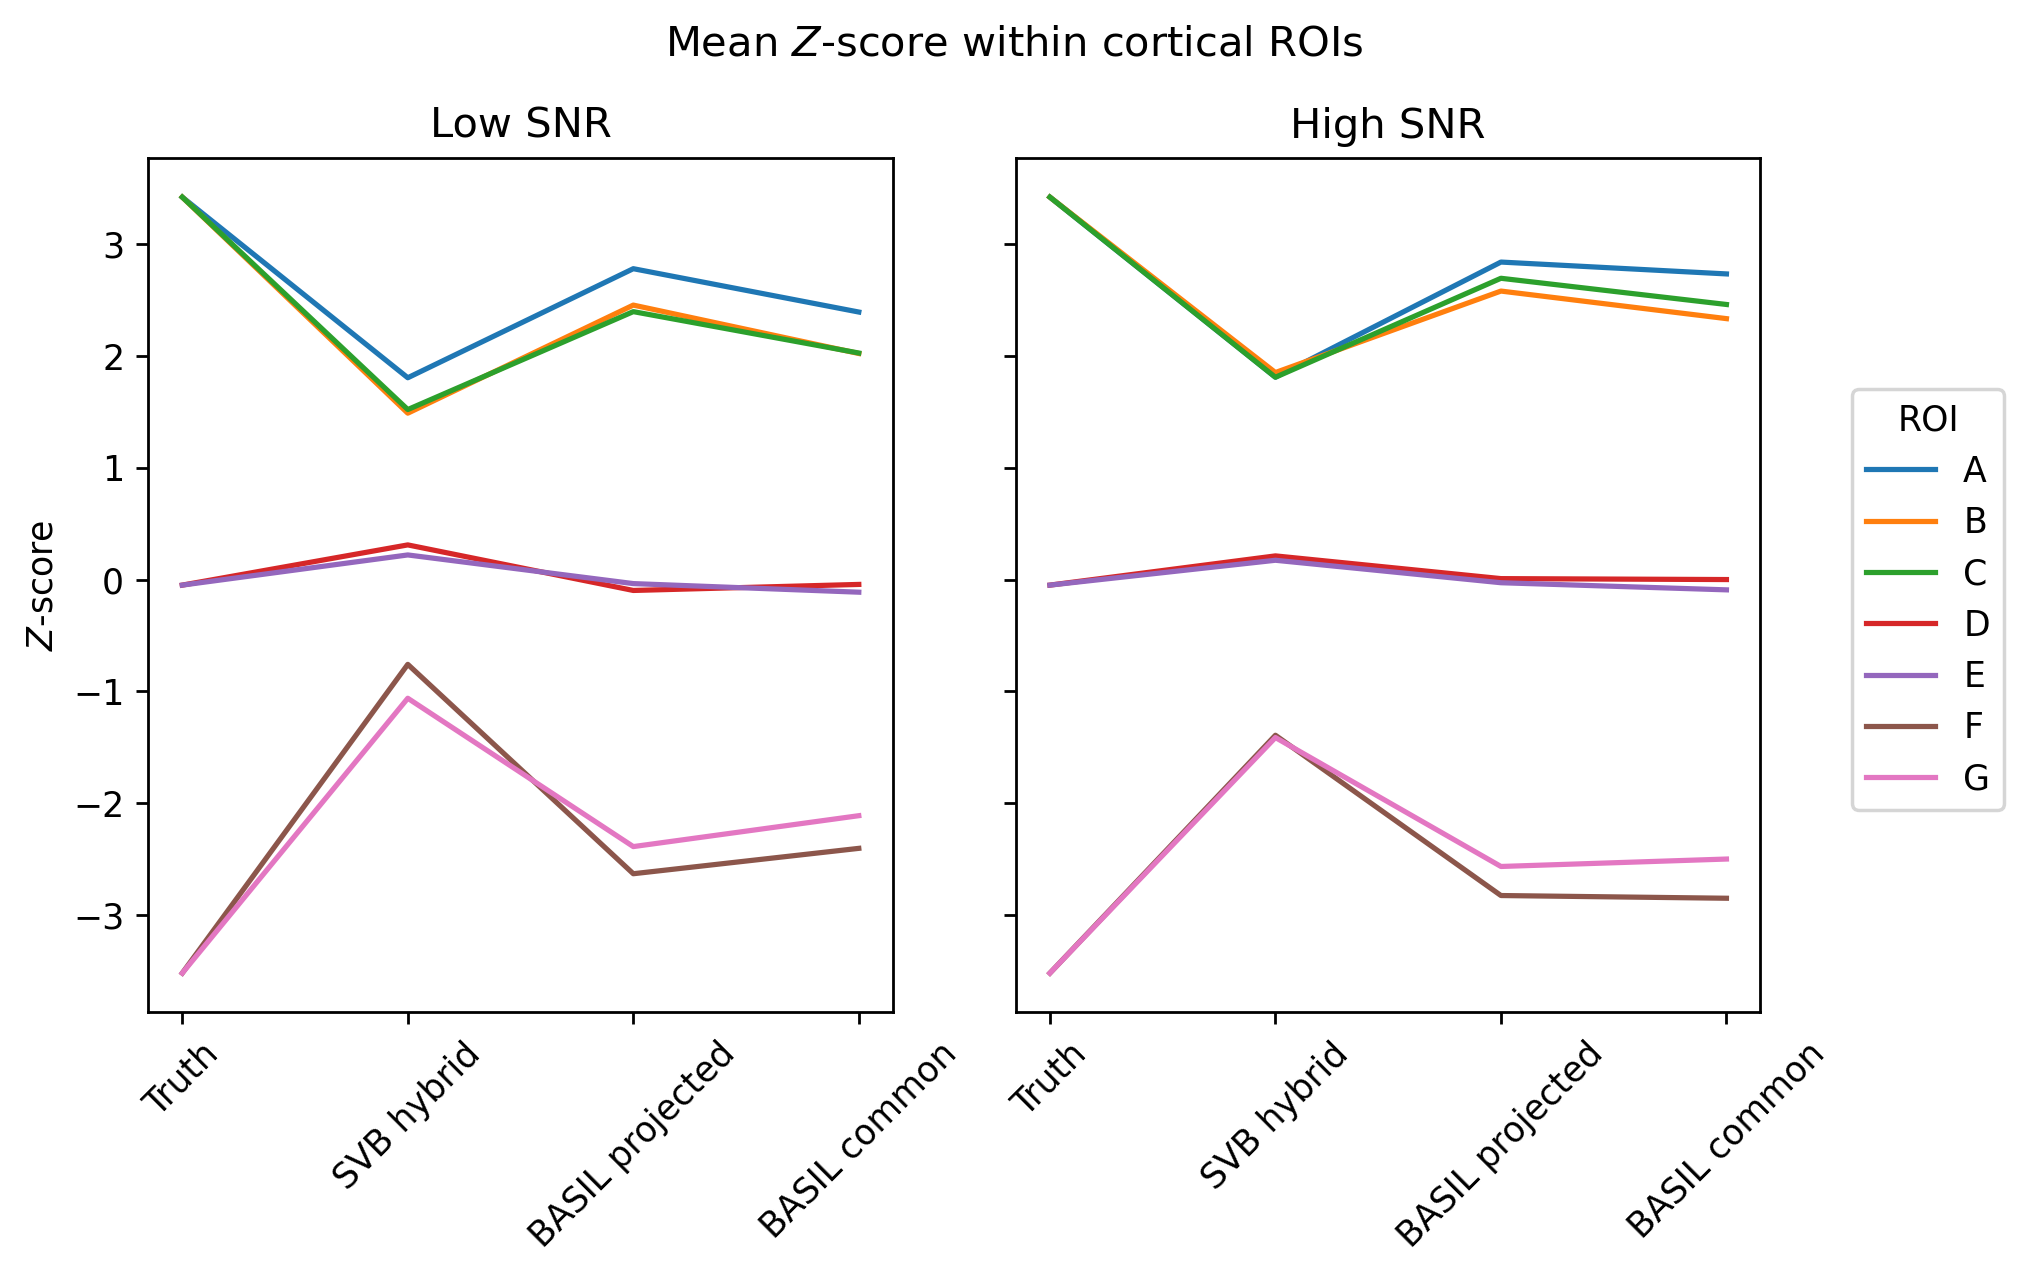
\includegraphics[width=\textwidth]{roi_zscores.png}
\caption{Mean $Z$-scores within ROIs. At high SNR, SVB was able to closely match ground truth, though again there was a positive bias in areas of hypo-perfusion. This was emphasised at low SNR, where in areas of hypo-perfusion the score was above -1. BASIL projected again showed good consistency across noise levels, which resulted in better performance than SVB at low SNR. Relative to BASIL projected, BASIL common suffered a reduced ability to estimate the full magnitude of ground truth scores.}
\label{roi_zscores} 
\end{figure}

Figure \ref{roi_zscores} shows mean $Z$-scores within cortical ROIs; ground truth values were approximately $\pm$3 for hypo/hyper-perfusion. At high SNR, SVB was able to reproduce positive scores almost exactly, but the presence of positive bias resulted in a substantially weaker score compared to ground truth in areas of hypo-perfusion. This effect was increased at low SNR, resulting in the near elimination of $Z$ in these areas. BASIL projected reproduced scores of around 1 smaller magnitude than truth (\textit{i.e.}, $\pm$2) and showed good consistency across noise levels; BASIL common showed a marginal further reduction in the ability to obtain the full magnitude of scores. 

\begin{figure}[H]
\centering
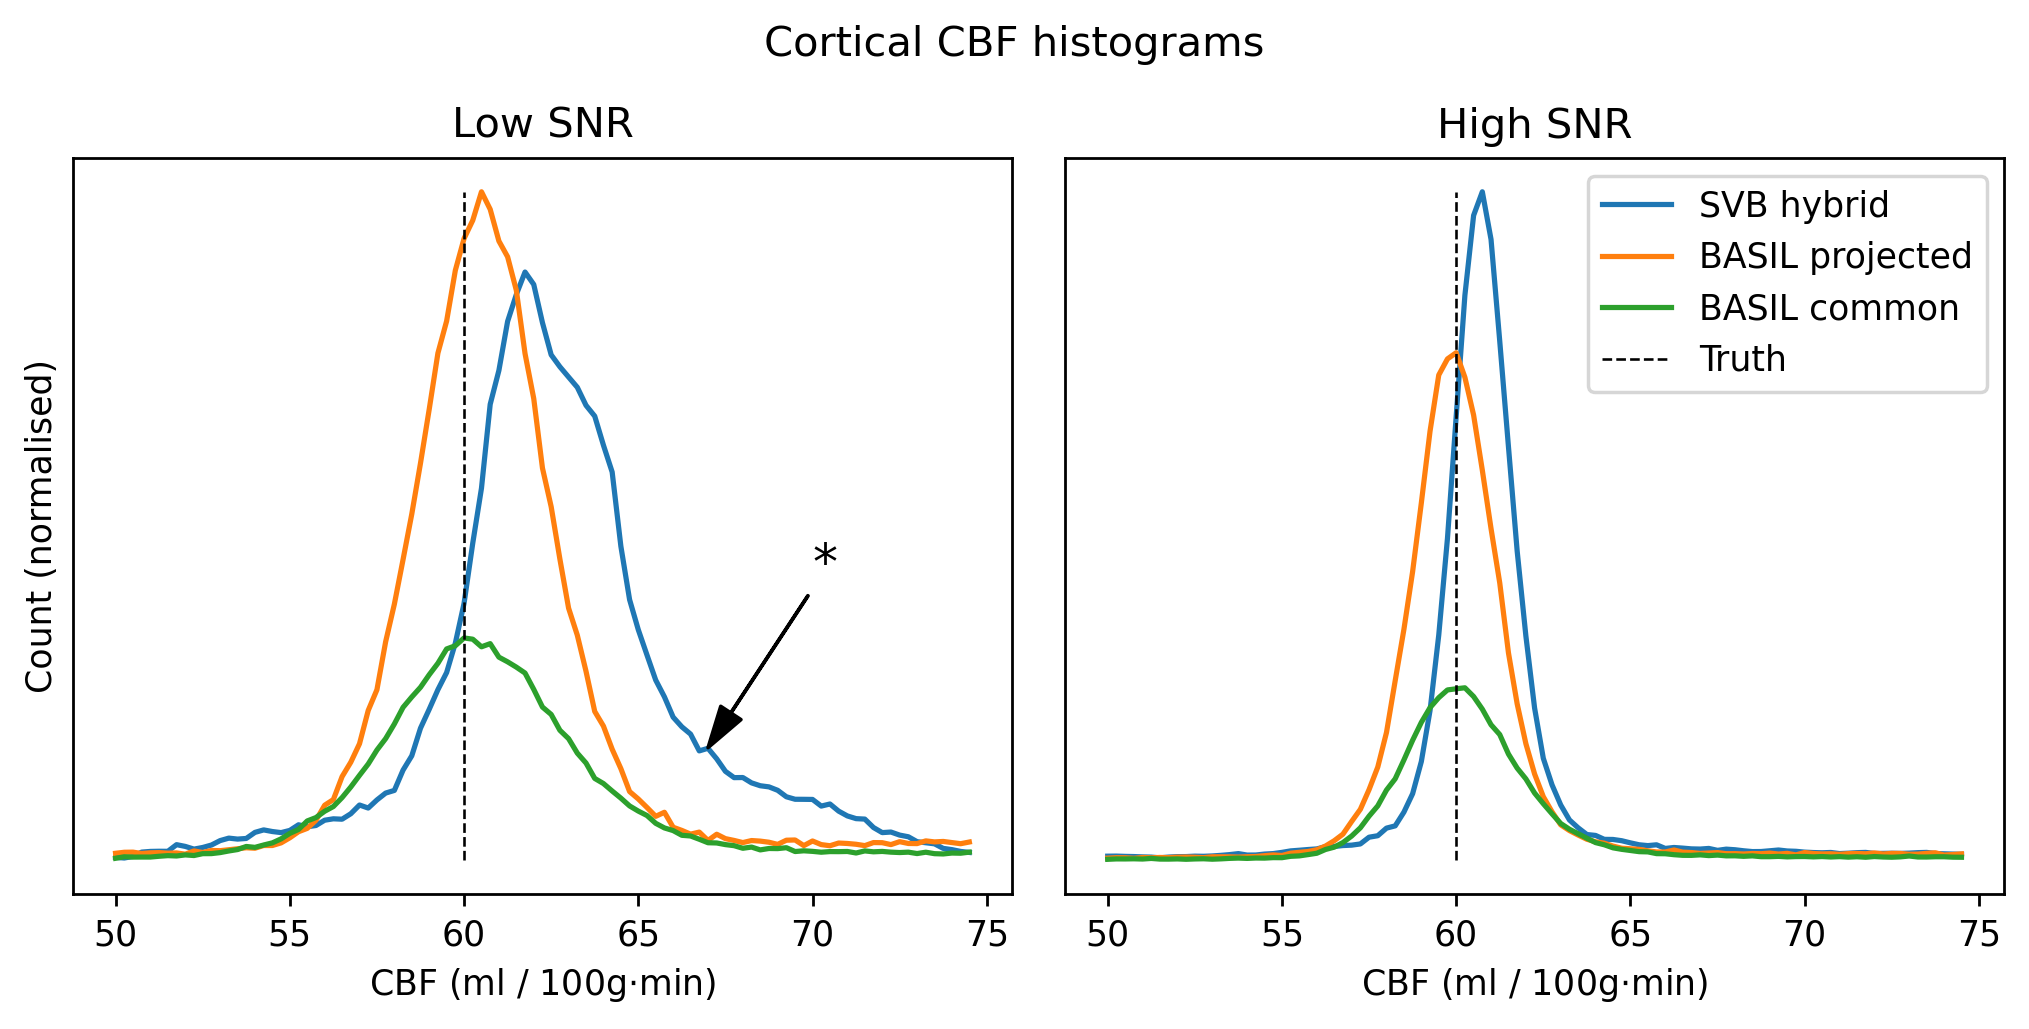
\includegraphics[width=\textwidth]{cortex_cbf_hist.png}
\caption{Histograms of cortical CBF. At both noise levels, the existence of a positive bias in SVB's estimates can be observed; at low SNR there was also a positive skew in the distribution (annotated with a star). Note that the data for BASIL common is volumetric in nature, not surface-based, which changes the total number of values in the histogram.}
\label{cortex_cbf_hist} 
\end{figure}

Figure \ref{cortex_cbf_hist} shows histograms of cortical CBF, aggregated across all repeats. The positive bias of SVB could be observed at both noise levels (the peak of the distribution was above ground truth in either case). By contrast, both variants of BASIL were essentially centred at the correct value. Furthermore, SVB's distribution at low SNR produced a positive skew. At high SNR, the strength of SVB's surface smoothing can be inferred from the low variance of the distribution. BASIL's common space result yielded the highest variance of all methods. 

\begin{figure}[H]
\centering
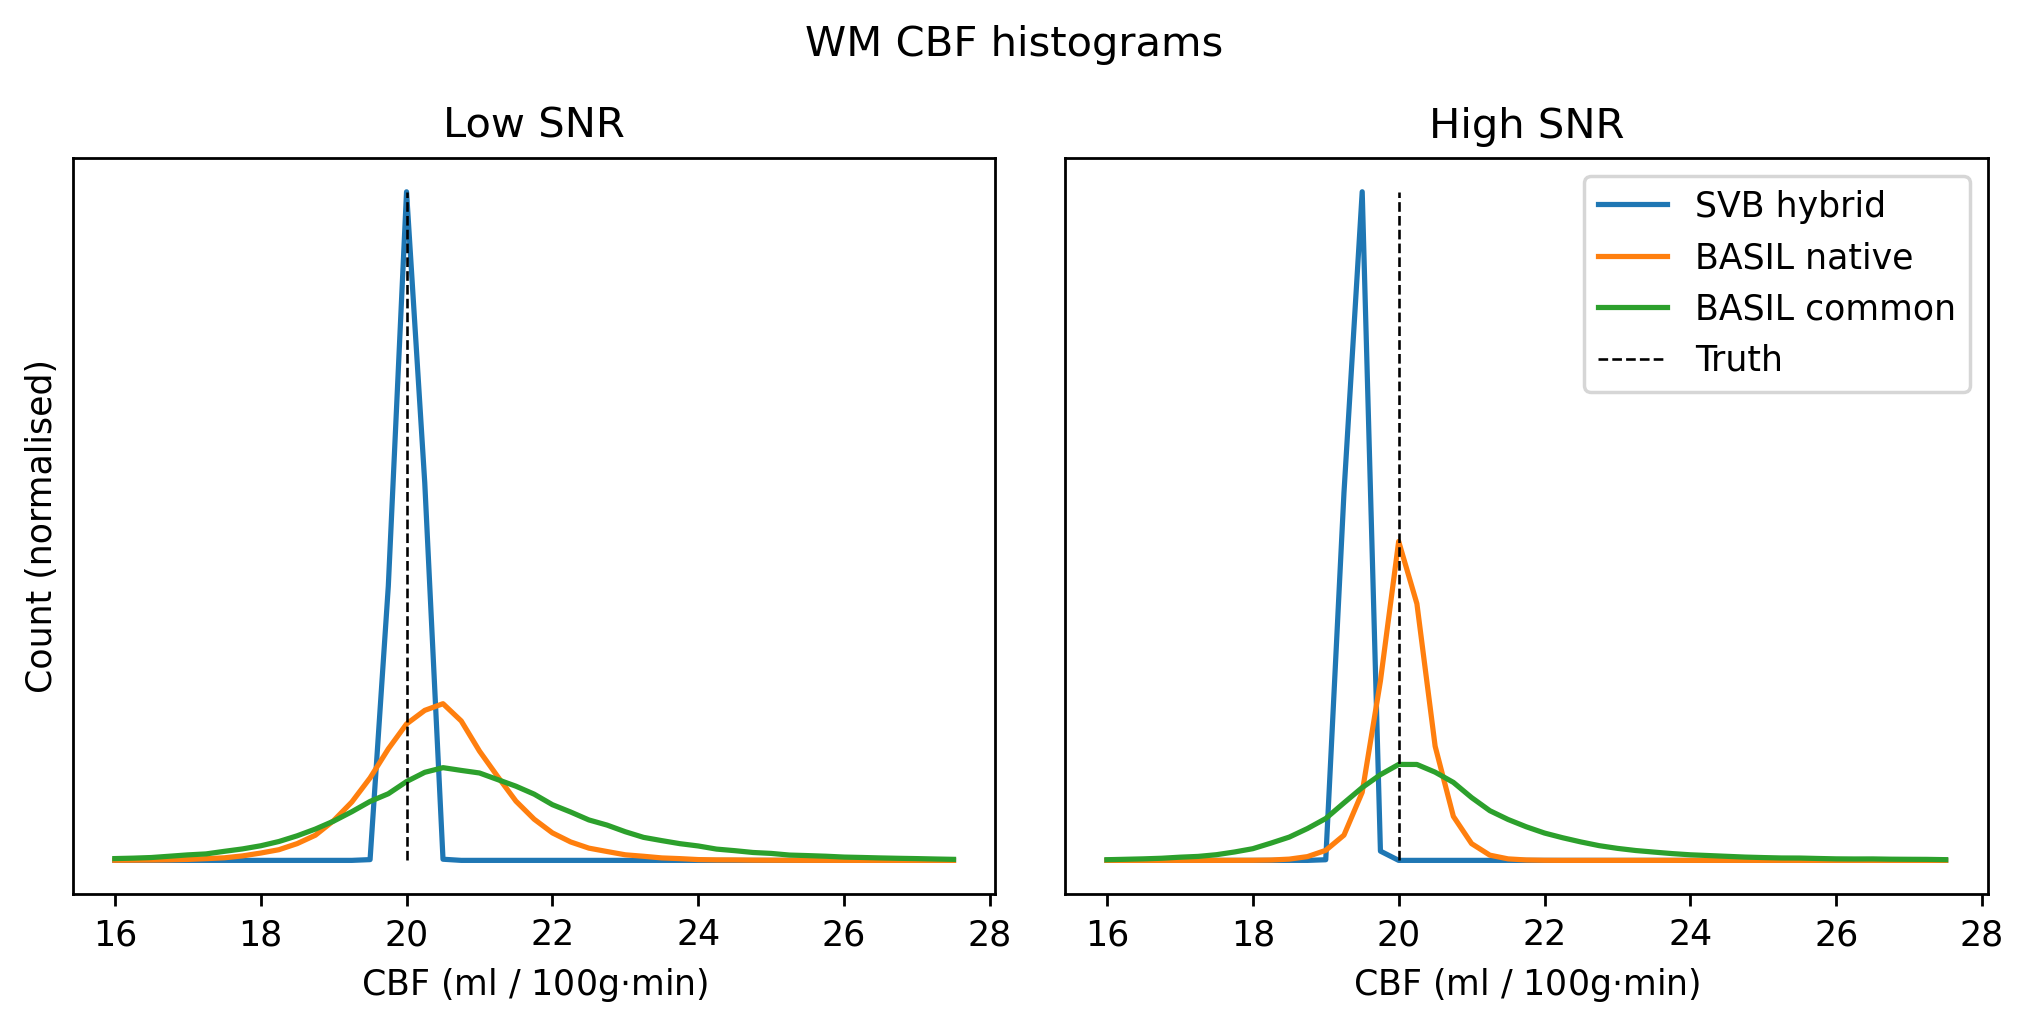
\includegraphics[width=\textwidth]{wm_cbf_dist.png}
\caption{Histograms of WM CBF (in volume space). SVB returned extremely tight distributions at both noise levels (the correct result); whereas there was no bias in the low SNR results, there was a negative bias in the high SNR case. BASIL native showed low bias in both cases, but also higher variance than SVB. BASIL common returned low bias and high variance in either case.}
\label{wm_cbf_dist} 
\end{figure}

Figure \ref{wm_cbf_dist} shows histograms of WM CBF (a volumetric quantity for all methods). SVB returned tight distributions at both noise levels, demonstrating high levels of volumetric smoothing in this parameter, and there was a small negative bias at high SNR. Both variants of BASIL demonstrated a small positive bias at low SNR; their variance was also substantially higher in either case. This indicates weaker volumetric smoothing of this parameter under BASIL than SVB. 

\subsection{Discussion}

The results presented here demonstrate both the promise and challenges of hybrid inference under SVB. Starting with the favourable case of high SNR data, SVB displayed the ability to reproduce areas of hyper- and hypo-perfusion with reasonable accuracy, whilst also returning close-to-correct estimates for other parameters of interest (\textit{i.e.}, constant WM CBF in the subcortex, though such a scenario may not be physiologically realistic). In this scenario, the main obstacle would seem to be the existence of low levels of bias in the estimates: referring to figure \ref{cortex_cbf_hist}, GM CBF was positively biased, whereas in figure \ref{wm_cbf_dist} WM CBF was negatively biased. On the cortical surface, this resulted in over-estimation in areas of hypo-perfusion. 

Moving onto the challenging case of low SNR data, the chief weaknesses of hybrid SVB observed here were the existence of substantial positive bias in cortical CBF and excessive levels of smoothing. Referring to the plots generated for the calibration of the volumetric spatial prior (figures \ref{parameter_noise} and \ref{acquisition_noise}), which demonstrated the existence of a relationship between the level of smoothing and bias in parameter estimates, it is likely that these two behaviours are linked and that the spatial prior is ultimately responsible. The presence of a positive skew in SVB's cortical CBF histogram (shown in figure \ref{cortex_cbf_hist}) will also have had a detrimental impact on its ability to obtain correct $Z$-scores in areas of hyper-perfusion (despite the \textit{absolute} estimates of CBF in these regions being approximately correct). 

Inference of CBF and ATT from noisy ASL data is a fundamentally challenging problem. The general kinetic model it itself symmetric in these two parameters: from an optimisation point of view, it is easy to trade off high CBF and long ATT for a lower CBF and shorter ATT if one has not sampled all regions of the kinetic curve (the two configurations are aliases of each other). Such behaviour was often observed in the course of development and is an argument in favour of returning to the use of a distributional prior on ATT\footnote{Though it was noted earlier that such an approach gave poor performance during development, so this should be regarded as an area of future work.}, as is used by BASIL. Further to this, the problem is only weakly determined in the case of multi-PLD data: two parameters must be estimated from $N$ PLDs of data-points; if volumetric PVEc under BASIL is to be performed then this becomes four parameters. In many regards, hybrid SVB exacerbates this problem. Though the definition of nodes in hybrid space does eliminate the redundancy inherent to BASIL of estimating GM and WM parameters in all voxels, regardless of whether the tissue in question is actually present there, in mixed cortical/subcortical voxels hybrid inference actually introduces \textit{more} nodes than BASIL. Recalling that the mean number of vertices enclosed within a cortical voxel for a 32k surface and 3mm isotropic voxel grid is around four, this implies that in the typical mixed voxel, ten total parameters will be estimated: eight from the surface and two for the subcortex. Hybrid inference therefore reduces the determinacy of the inference problem compared to volumetric. 

In light of this, it is easy to understand why the spatial prior should play such a vital role in surface inference. With infinitely many possible configurations of ten parameters, for example, that successfully reconstruct the data acquired in a given voxel, the prior plays a key role in ensuring that only plausible solutions are selected. In quantitative terms, this could readily be observed in the evolution of different components of the optimisation cost throughout the inference process, shown in figure \ref{optimisation_cost} for a single repeat of low SNR data (note that the spatial prior was enabled on all parameters, and therefore represents the only contribution to latent cost). 

\begin{figure}[H]
\centering
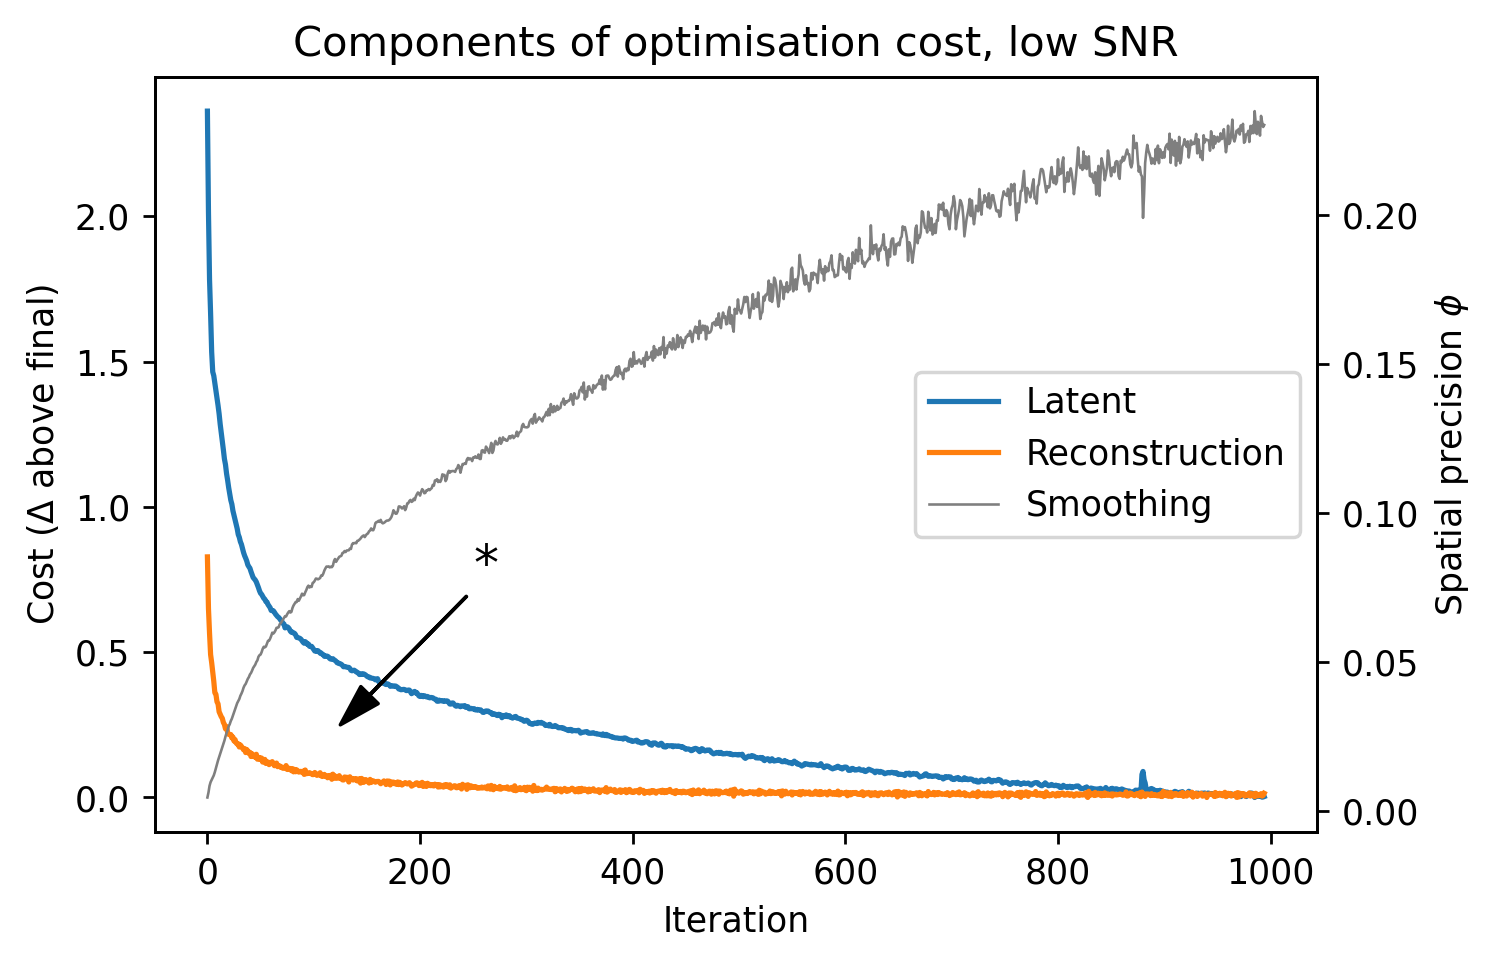
\includegraphics[width=0.8\textwidth]{optimisation_cost.png}
\caption{Evolution of optimisation cost throughout inference on a single repeat of low SNR data. Reconstruction cost attained its final value within 200 epochs, whereas latent cost (a function of smoothing) continued to fall throughout, while $\phi$ increased monotonically. The annotated region denotes epochs where reconstruction cost was already minimal but latent cost continued to fall; it is suspected this is where excessive smoothing takes place.}
\label{optimisation_cost} 
\end{figure}

The objective of optimisation is to maximise the free energy, which itself may be separated into reconstruction and latent cost terms. Figure \ref{optimisation_cost} shows that reconstruction cost quickly fell to its ultimate value within around 200 epochs, whereas latent cost continued to fall throughout optimisation (whilst the smoothing parameter $\phi$ increased continually). It is argued that this behaviour represents `shuffling signal around': the optimisation is quickly able to find a configuration of parameters that accurately reconstructs the data, but then spends the remaining epochs shuffling these values between neighbouring nodes. Given the corresponding increases in $\phi$, the optimiser has tended towards fundamentally smooth parameter configurations. 

A final discussion point regarding the differences between BASIL's and SVB results concerns the nature in which they perform optimisation. For BASIL, a series of analytic update equations are derived using the calculus of variations and many assumptions or simplifications can be `baked in' during this process (for example, linearisation of the generative model). SVB does not make any similar assumptions or modifications and as a result it is reasonable to question whether its optimisation is more unconstrained as a result. Especially at higher learning rates, SVB exhibited a willingness to visit negative regions of parameter space and the use of distributional priors was not sufficient to preclude this. As a result, the spatial prior was used on both CBF and ATT, with the clear drawback of applying excessive amounts of smoothing in most scenarios. It would be beneficial to further investigate this topic and to determine to what extent the differences between BASIL and SVB are fundamental in nature. 

The drawbacks of searching for surface-oriented features (areas of hypo- and hyper-perfusion) in a volumetric manner were demonstrated by the results produced by BASIL common. Though subtle, they were nevertheless clear: a reduced ability to obtain the full parameter range of the ground truth data (difference between maximum and minimum) and reduced magnitude of $Z$-scores. These can be attributed in part to the drawbacks inherent to the volumetric approach (though difficult to quantify), and in part to the drawbacks of performing analysis in a common aligned space. For the former, such topics have been investigated in much greater detail by proponents of the surface-based approach (for example, \cite{Coalson2017}), whereas for the latter the results presented earlier in chapter \ref{pvec_chapter} serve as justification for this assertion. In particular, registration of ASL data before parameter estimation serves to increase PVE in an unpredictable manner that cannot be fully accounted for in later processing. This in turn increases the variance of parameter estimates, which in the course of the experiments presented in this chapter, led to reductions in the magnitude of $Z$-scores. 

\section{Future work}
\label{svb_future}

In light of the results presented in this chapter, it is suggested that future work should question whether the spatial prior is in fact necessary in surface space. This argument is constructed in two parts. 

Firstly, recall the assertion that the prior solves the inherently under-determined problem of parameter estimation in voxels that contain multiple tissues. In doing so, the spatial prior provides a form of \textit{spatial regularisation} \cite{Groves2009a}, and it is the latter mechanism that actually resolves the under-determinacy. The linear regression method for PVEc provides an explicit formulation of the fact that data from multiple voxels is required in such a situation. Further, it is noted that the role of the prior in volume space is to link a node of estimation (a voxel centre) to multiple \textit{data points} (other voxels). Simply linking nodes to other nodes in and of itself is of no consequence to the determinacy of the overall problem; the conditioning provided by the prior follows from the fact that nodes are linked to multiple data points (and it so happens that there is a one-to-one correspondence between nodes and voxels in volume space). This ties into the reasoning behind the discriminated Laplacian in surface space: node connections within voxels are of different utility to node connections between voxels. 

Secondly, analysis of the surface to volume projection matrix for a typical 32k cortical surface and 3mm isotropic voxel grid reveals that this operation is in fact comfortably over-determined. Each element within the projection matrix denotes the contribution that vertex $i$ makes to voxel $j$. Counting the number of voxels that each vertex contributes to yields the histogram presented in figure \ref{vox_per_vtx}. 

\begin{figure}[H]
\centering
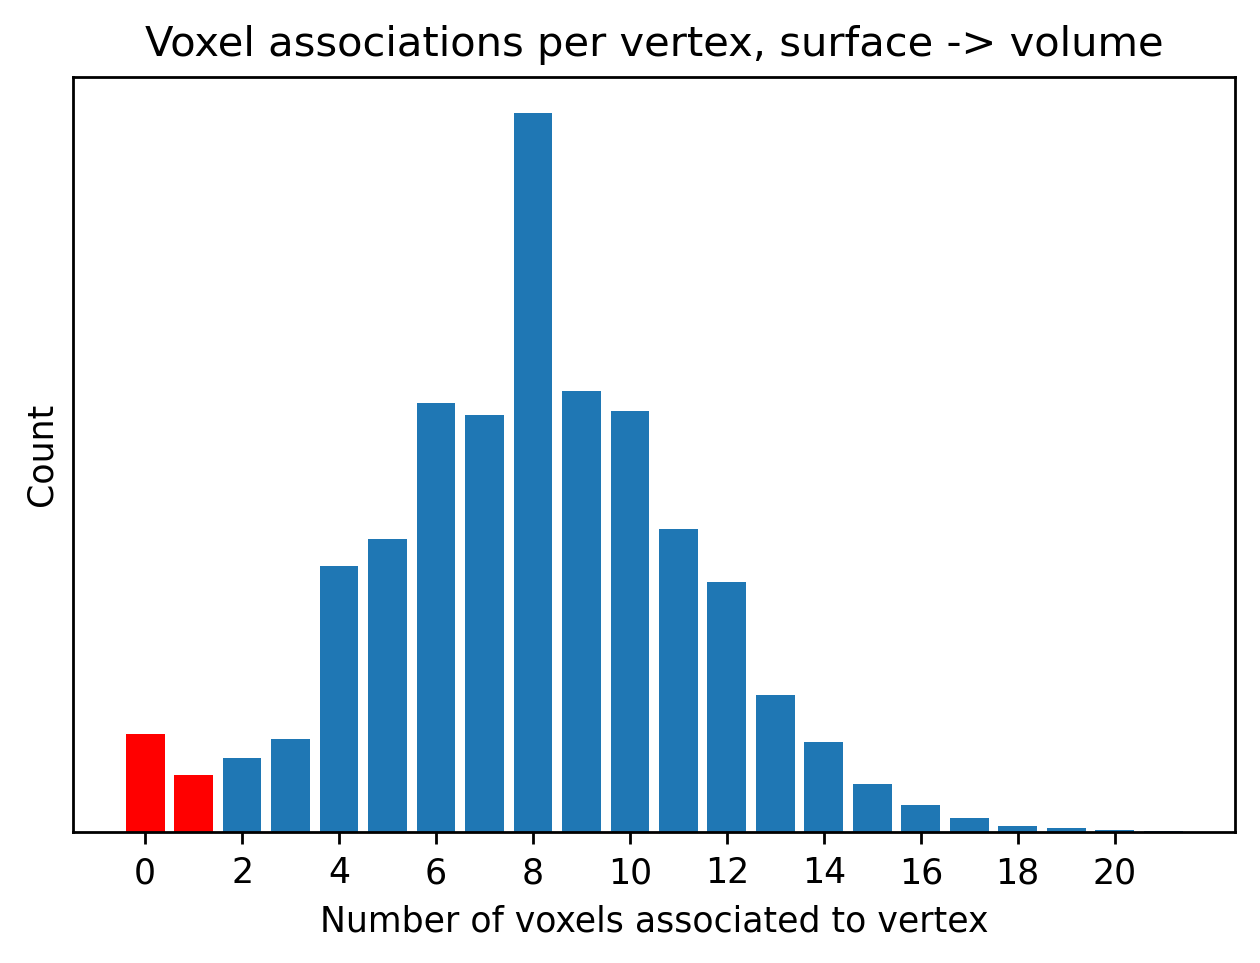
\includegraphics[width=0.7\textwidth]{vox_per_vtx.png}
\caption{Histogram of the number of voxels associated to each surface vertex. The vast majority of vertices are associated to two or more voxels; the small number associated to one or fewer are highlighted in red. It is suspected that only these vertices suffer from the issues of being under-determined.}
\label{vox_per_vtx} 
\end{figure}

The mean number of voxels associated to each vertex is just over eight, and the overwhelming majority of vertices are associated to at least two voxels. In effect, what the histogram reveals is that a high degree of smoothing is already factored into the projection: a given vertex contributes to multiple different voxels, which in turn means its overall weight to any individual voxel within the data reconstruction is diffuse. 

From the point of view of determinacy, it is argued that the only vertices that pose a challenge are those associated to one or fewer voxels\footnote{Note that an association to zero voxels arises when the GM PV in the voxel is negligible, for example around the corpus callosum where the cortex has no defined thickness.}. This can be understood by considering the alternative situation: a vertex that is associated to many voxels cannot plausibly be assigned an extreme value because it must successfully reconstruct many data points. In contrast, a vertex that is associated to only a single voxel can freely be assigned an extreme value with little consequence. Other vertices in the neighbourhood will see their values change by a corresponding amount to offset this, but when this is spread over multiple vertices the individual changes will be small, and therefore of little consequence to the voxels that those vertices are further associated to. Hence, even with an extreme vertex value in the neighbourhood, a plausible reconstruction of the data may be obtained in that individual voxel. 

Thus, it is argued that figure \ref{vox_per_vtx} demonstrates that a degree of spatial regularisation is in fact already incorporated into the surface to volume projection that forms part of SVB hybrid inference. Though this is not the same as a spatial prior \textit{per se}, the consequence (regularisation) is nevertheless similar: to mitigate the under-determined nature of inference, the key metric is the number of data points to which each node is linked; the histogram shows that most vertices are in fact already linked to a high number of voxels before application of the prior. Following this chain of reasoning, the underwhelming results and excessive smoothing observed with application of the prior on the surface make sense: the prior adds minimal information and serves only to artificially increase the level of smoothing that is already intrinsic to the projection. 

The hypothesis that a high level of smoothing is already inherent to the surface to volume projection may be investigated by running SVB inference without the spatial prior on the surface. Simulated multi-PLD ASL data of very high SNR (properties as set out in section \ref{pvec_chapter_sim_data}) was used; constant parameter values for CBF and ATT were assumed. Alongside parameter estimates, SVB returns posterior variances at all nodes, which may be regarded as a measure of uncertainty (and in turn as a rough proxy for under-determinacy). Variance in CBF estimates on the surface is shown in figure \ref{var_at_vtx}. 

\begin{figure}[H]
\centering
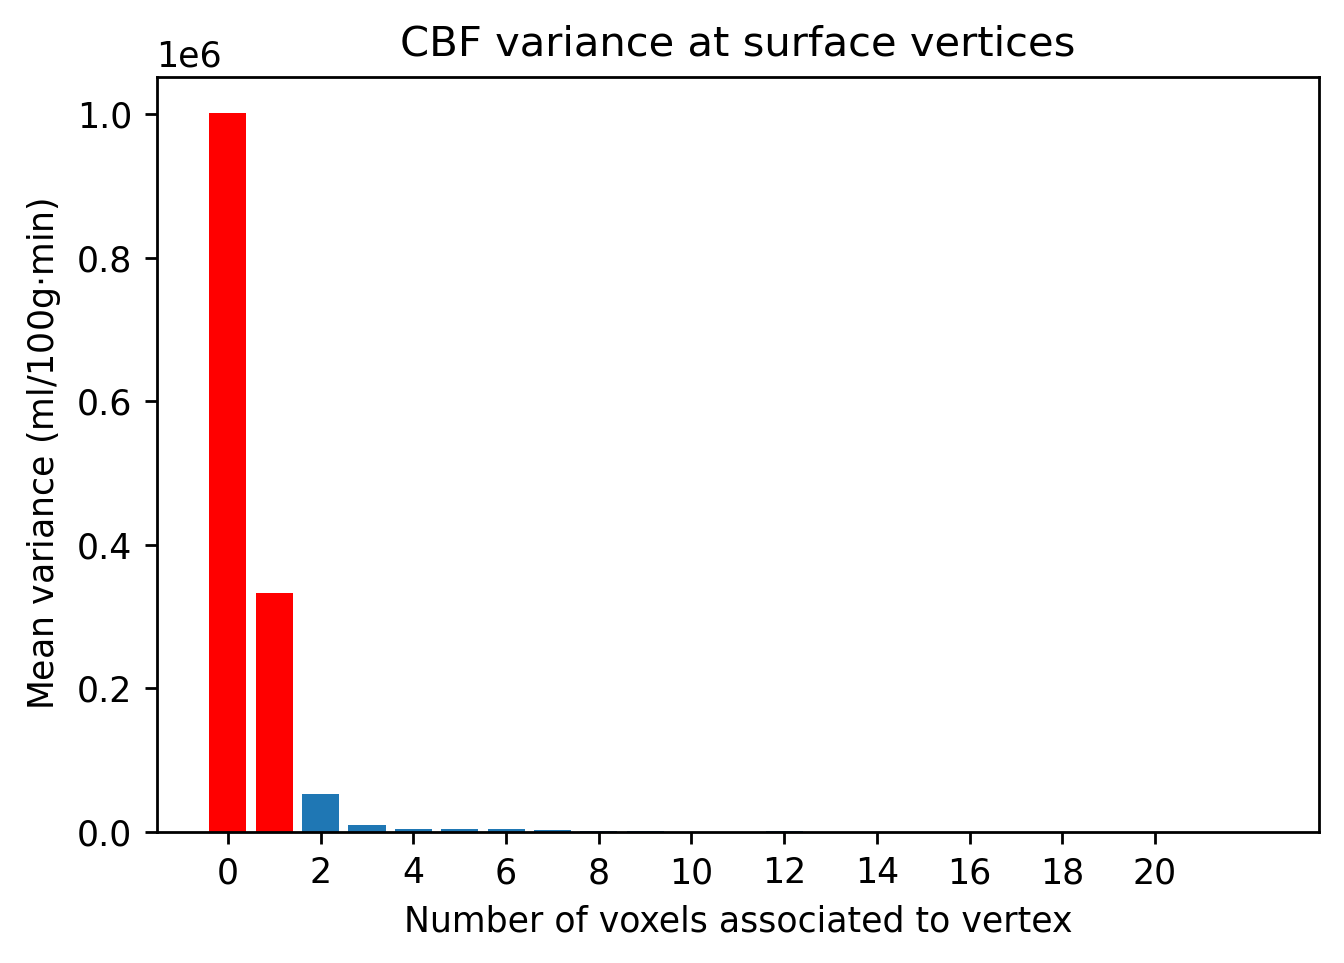
\includegraphics[width=0.7\textwidth]{var_at_vtx.png}
\caption{CBF posterior variance at surface vertices, sorted by number of associated voxels. The mean variance across vertices in each bin is shown. Posterior variance may be interpreted as parameter uncertainty, and in turn as a proxy for the extent of under-determinacy at that vertex. Vertices with one or fewer associated voxels (highlighted in red) accounted for almost all variance; voxels that are comfortably over-determined returned comparatively low variance.}
\label{var_at_vtx} 
\end{figure}

Figure \ref{var_at_vtx} was generated by sorting surface vertices into bins according to the number of voxels to which they are associated (the same basis as for the histogram in figure \ref{vox_per_vtx}). The mean variance across vertices was then taken within bins. The plot demonstrates that the overwhelming majority of parameter uncertainty is concentrated on vertices with one or fewer voxel associations. It is suspected that this is a direct consequence of their under-determined nature: in effect, the optimisation has acknowledged that it could assign them almost any value with little penalty for doing so. 

In light of this analysis, the suggested solution for the application of the spatial prior on the surface is to restrict it to only those vertices that are actually under-determined. This could be achieved by modifying the Laplacian operator to ignore all connections between vertices with $n$ or more associated voxels. At a cursory inspection, it may be that vertices with two associated voxels are only weakly determined and also require the prior (they show some uncertainty on figure \ref{var_at_vtx}); but it is equally possible that second-order effects may take care of this. For example, once the vertices with one or fewer voxel associations are properly conditioned, this may have a beneficial spillover effect for all other vertices associated to the same voxel. 

\section{Conclusion} 

An implementation of simultaneous and combined surface and volumetric inference under a stochastic VB framework (hybrid SVB) has been presented. Adaptations to existing volumetric implementations of VB were required to enable hybrid inference, most notably to the spatial prior; the inclusion of a projection from the space of inference into the data (volumetric) space; and the inclusion of acquisition noise as a purely volumetric parameter. In order to implement said projection, hybrid SVB is intimately tied to the Toblerone projection framework introduced in chapter \ref{projection_chapter}. 

Substantial changes have been made to the spatial prior within hybrid SVB because a direct transplant of FABBER's implementation was found to give suboptimal performance. Though these changes can be justified in theoretical terms (for instance, the different strength of belief regarding similarity for within- or between-voxel connections), their implementation and inclusion thus far has been undeniably empirical in nature. A simple calibration involving representative ASL data has yielded a configuration that gives plausible parameter estimates, but the presence of bias and excessive smoothing at low SNR shows that further work on this front is required. Nevertheless, such a process is not entirely out of step with the previous literature on the spatial prior within VB: Penny \textit{et al.} did envisage this topic being revisited as experience in applying the prior to physiological data accumulates \cite{Penny2005}. 

In a broad sense, hybrid SVB inference can be said to work on ASL data. Given data of favourable SNR, it was able to reproduce areas of hyper- and hypo-perfusion, not withstanding the aforementioned existence of low levels of bias. In particular, the fact that it was better able to recover absolute values of hyper-perfusion compared to BASIL is promising, given that the high PVE inherent to imaging the cortex is one of the key weakness of a volumetric approach. With the introduction of increasing levels of noise, however, performance degraded such that volumetric approaches were found to function better. Given the metrics on which performance suffered (increasing bias, a skew in the distribution of estimates, excessive smoothing) it is suspected that the spatial prior is ultimately responsible. This assertion is made in light of the fact that the calibration experiments revealed a bias-variance relationship, where variance represents a proxy measure of smoothing. As such, future work should investigate the extent of spatial regularisation and conditioning required for successful inference, and whether modifications to the spatial prior in surface space may help achieve this. 

